% =====================================================================
%  The Geometry and Transfer of RLVR in Small Reasoning Models
%  TMLR / arXiv draft
%
%  TEMPLATE: official TMLR style (tmlr.sty, tmlr.bst, fancyhdr.sty in this dir).
%  Switch mode via the class option on \usepackage{...}{tmlr}:
%    \usepackage{tmlr}            -> submission   (anonymous, "Under review" banner)
%    \usepackage[preprint]{tmlr}  -> arXiv preprint (named authors, no banner)  [CURRENT]
%    \usepackage[accepted]{tmlr}  -> camera-ready (named authors + OpenReview line)
%  tmlr.sty already provides: natbib, fontenc[T1], lmodern, fancyhdr, page geometry.
% =====================================================================

\documentclass{article}
\usepackage[preprint]{tmlr}

% packages tmlr.sty does not already provide:
\usepackage{amsmath,amssymb,amsfonts}
\usepackage{graphicx}
\usepackage{booktabs}
\usepackage{array}
\usepackage{multirow}
\usepackage{xcolor}
\usepackage{caption}
\usepackage{subcaption}
\usepackage{microtype}
\usepackage{pifont}
\usepackage{url}
\usepackage[hidelinks]{hyperref}
\captionsetup{font=small}
\graphicspath{{figures/}}
\newcommand{\tv}{\tau}
\newcommand{\Wsft}{W_{\mathrm{SFT}}}
\newcommand{\Wg}{W_{\mathrm{GRPO}}}
\newcommand{\dg}{^{\circ}}
\newcommand{\cmark}{\ding{51}}
\newcommand{\xmark}{\ding{55}}
\renewcommand{\arraystretch}{1.08}

\title{The Geometry and Transfer of RLVR in Small Reasoning Models}

\author{%
  \name Sunny Guha\thanks{Work done outside the affiliated institutions.} \email email TBD \\
  \addr Oracle
  \AND
  \name Chaitanya Afle$^{*}$ \email email TBD \\
  \addr Cranium.ai
}

\begin{document}
\maketitle

\begin{abstract}
Reinforcement Learning with Verifiable Rewards (RLVR) is now the default recipe for eliciting
reasoning in language models, yet its training dynamics in \emph{small} reasoning models remain
comparatively under-studied; we use GRPO across ten \texttt{reasoning-gym} tasks to ask two
questions: how RLVR \emph{transfers} across tasks, and what it does to a model's
\emph{weight-space geometry}.
\textbf{Transfer.} RLVR is not a universal improver. Across a $10\times 10$ cross-task transfer
matrix evaluated at four model scales, GRPO degrades $36\%$ of (train, eval) task pairs, with
catastrophic cross-task drops of up to $-52$ points. Learning rate, not model size, is the
controlling hyperparameter, and arithmetic degrades at every scale.
\textbf{When RLVR helps.} To predict \emph{when} RLVR helps, we introduce the \emph{Atomic
Readiness Score} (ARS), a $\sim$1-GPU-hour zero-shot probe that decomposes a task into grounding
(L1) and local-reasoning (L2) atoms. From these atoms, ARS recommends one of three training
regimes (Direct, Atomic-Only, Atomic-Warm) before any GRPO run. It selects the optimal regime on
$6/7$ tasks, and its single failure is mechanistically diagnostic rather than random.
\textbf{Geometry.} The task vector $\tau = \Wg-\Wsft$ carries a scale- and family-invariant
signature: GRPO preserves $W$'s spectrum, $\tau$ is near-orthogonal to $W$'s top subspace, and the
\texttt{mlp.down\_proj} basis is \emph{frozen} ($0\dg$ rotation) while
\texttt{mlp.up\_proj}/\texttt{attn.q\_proj} rotate $1.5\dg$--$2.7\dg$, growing monotonically with
scale. The rotation \emph{magnitude} is identical for every task (per-task spread $\leq0.06\dg$):
GRPO spends a fixed per-layer rotation budget regardless of what it learns, and tasks differ only in
the \emph{direction} of that rotation and the network \emph{depth} at which each writes its change,
with the depth shift across scale itself task- and family-dependent. This geometry delivers one universally safe task-arithmetic merging recipe across 19
pairs (discard \texttt{mlp.down\_proj} contributions: 40/48 cells lossless), shows simple summation
beats $1/N$ averaging, and that atomic- and direct-trained vectors compose in distinct but
cross-scale-stable ways. It does not, however, buy prospective predictability: two merge predictors
strong at $n{=}7$ (weight-space sign-agreement $r{=}{-}0.81$, behavioral L1-grounding
$r{=}{-}0.76$) both collapse at $n{=}19$ ($-0.27$ and $+0.06$), and merge-compatibility is
\emph{pair-dependent}, not task-intrinsic. We argue these honest negatives are a contribution: the
field has implicitly assumed task-intrinsic merge structure and cheap pre-probes, and our evidence
rules out both for reasoning RLVR vectors. We release all checkpoints, probes, and analysis code.
\end{abstract}

% =====================================================================
\section{Introduction}
% =====================================================================
Reinforcement Learning with Verifiable Rewards (RLVR), typically Group Relative Policy
Optimization \citep{shao2024deepseekmath} with a binary correctness reward, has become the
standard tool for turning a pretrained language model into a reasoner
\citep{deepseekai2025r1}. Most of the public understanding of RLVR comes from \emph{large}
models, where it reliably helps. For \emph{small} models (here $\leq 8$B), the picture is
murkier, and practitioners often treat GRPO as a monotone improvement operator: run it on a
task, get a better model. This paper is a systematic, multi-phase rebuttal of that assumption,
and an attempt to replace it with a mechanistic account of what GRPO actually \emph{does} to a
small model's weights and capabilities.

We organize the study as four interlocking phases, each answering a distinct question and
feeding the next:

\begin{enumerate}
\item \textbf{Does single-task GRPO transfer (Phase~1)?} We build full $10\times10$ transfer
matrices at 3B/4B/7B/8B. GRPO helps some tasks dramatically (countdown $+60$ at 7B) but
\emph{degrades $36\%$} of (train, eval) pairs, sometimes catastrophically ($-52$).
Learning rate, not scale, is the dominant control.
\item \textbf{Can a cheap probe predict the right RLVR regime (Phase~2)?} We decompose each
task into atomic sub-skills and define the Atomic Readiness Score (ARS). ARS predicts the
best of \{Direct-RLVR, Atomic-Only, Atomic-Warm\} on $6/7$ tasks, and the one miss
(\texttt{mini\_sudoku}) pinpoints \emph{why} the framework can fail.
\item \textbf{What does GRPO do to the weights (Phase~3)?} We characterize the task vector
$\tau=\Wg-\Wsft$ geometrically. GRPO has a universal structural signature (spectrum-preserving,
\texttt{mlp.down\_proj}-basis-frozen, feature-projector rotations of $1.5\dg$--$2.7\dg$) whose
\emph{magnitude} is the same for every task, a fixed per-layer rotation budget, and a task-specific
\emph{location}: which depths each task rotates and in which direction, with the depth shifting
task- and family-dependently across scale.
\item \textbf{Can task vectors be merged into multi-skill models (Phase~4)?} The Phase-3
geometry motivates task-arithmetic merging. We find one universally safe recipe and a clean
training-regime effect, but we also show, on an expanded $n{=}19$ sample, that every cheap
\emph{prospective} predictor of merge damage we tried (including two we initially believed at
$n{=}7$) fails, and that merge compatibility is a property of the \emph{pair}, not the task.
\end{enumerate}

\paragraph{Contributions.}
(i) The first large cross-scale RLVR transfer matrix for small models, establishing that GRPO
is not free improvement and that LR dominates scale (\S\ref{sec:phase1}).
(ii) ARS, a $\sim$1-hour zero-shot diagnostic that selects the RLVR regime, validated on $6/7$
tasks, plus craft lessons (long-answer atoms, single hard difficulty transitions, the harm of
partial credit) from a 15-condition shortest-path study (\S\ref{sec:phase2}).
(iii) A scale- and family-invariant geometric signature of GRPO updates, including the
\texttt{mlp.down\_proj}-frozen invariant and a fixed per-layer rotation budget that every task spends
identically (verified per task) and redirects only in rotation direction and network depth
(\S\ref{sec:phase3}).
(iv) A practical, geometrically motivated merge recipe; a cross-scale-stable atomic-vs-direct
composition effect; and a rigorously documented \emph{null-predictor catalogue} that corrects
two of our own earlier ($n{=}7$) claims (\S\ref{sec:phase4}).
We view (iv)'s honest negatives, surviving expansion to $n{=}19$, as a first-class
contribution to a literature that has assumed the opposite.

% =====================================================================
\section{Related Work}
% =====================================================================
\paragraph{RLVR and GRPO.} GRPO \citep{shao2024deepseekmath} replaces PPO's
\citep{schulman2017ppo} learned value function with a group-relative advantage, and underlies
recent reasoning systems \citep{deepseekai2025r1}. DAPO \citep{yu2025dapo} refines the loss
(decoupled clipping, dynamic sampling); we use the DAPO variant with $\beta{=}0$ throughout.
Prior work studies RLVR at scale; we instead ask what it does \emph{mechanistically} to small
models, where its failure modes are visible.

\paragraph{Curriculum and decomposition.} Curriculum learning \citep{bengio2009curriculum}
orders examples of the \emph{same} task by difficulty; least-to-most and chain-of-thought
prompting \citep{zhou2023leasttomost,wei2022cot} decompose at inference time with no training
signal. Our atomic curriculum (Phase~2) instead \emph{trains} on categorically distinct
prerequisite sub-skills with verifiable rewards, and uses a pre-training probe (ARS) to decide
\emph{whether} decomposition will help.

\paragraph{Task arithmetic and model merging.} Editing models with task arithmetic
\citep{ilharco2023editing}, TIES-Merging \citep{yadav2023ties}, DARE \citep{yu2024dare},
model soups \citep{wortsman2022modelsoups}, and Fisher-weighted averaging
\citep{matena2022fisher} merge fine-tuned checkpoints by combining weight deltas. This
literature largely studies supervised/instruction vectors and assumes that merge compatibility
can be predicted or repaired by sparsification/sign-resolution heuristics. Phase~4 stress-tests
these assumptions specifically for \emph{RLVR} vectors on reasoning tasks and finds the
prospective-prediction premise unsupported at $n{=}19$.

\paragraph{Geometry of fine-tuning.} Low intrinsic dimensionality \citep{aghajanyan2021intrinsic},
LoRA \citep{hu2022lora}, and orthogonal fine-tuning \citep{qiu2023oft} argue that adaptation
lives in a small or rotation-like subspace. Phase~3 shows GRPO exhibits this pattern unusually
strongly (spectrum-preserving, near-orthogonal $\tau$) and localizes it to specific layer types,
which directly informs the merge recipe of Phase~4.

% =====================================================================
\section{Experimental Setup}
\label{sec:setup}
% =====================================================================
\paragraph{Models.} We study four post-SFT checkpoints spanning two Qwen families and four scales
(Table~\ref{tab:models}). The Qwen2.5/Qwen3 split (3B/7B vs.\ 4B/8B) is a family confound we cannot
fully disentangle from scale and flag throughout. Before any RL, each base is SFT'd for 3 epochs
($\mathrm{lr}{=}2\!\times\!10^{-5}$) on 1{,}000 \emph{task-agnostic} warm-up samples (trivia, unit
conversions, word puzzles, date reasoning) to teach the structured
\texttt{<think>...</think><answer>...</answer>} contract; the data is deliberately task-agnostic so
no \texttt{reasoning-gym} task gains an advantage. These $\Wsft$ checkpoints are the reference point
throughout.

\begin{table}[h]
\centering\small
\caption{The four models. Qwen3 has no separate \texttt{-Instruct} variant; its base already
follows instructions.}
\label{tab:models}
\begin{tabular}{llll}
\toprule
Scale & Family & Params & HuggingFace ID\\
\midrule
3B & Qwen2.5 & 3B & \texttt{Qwen/Qwen2.5-3B-Instruct}\\
4B & Qwen3   & 4B & \texttt{Qwen/Qwen3-4B}\\
7B & Qwen2.5 & 7B & \texttt{Qwen/Qwen2.5-7B-Instruct}\\
8B & Qwen3   & 8B & \texttt{Qwen/Qwen3-8B}\\
\bottomrule
\end{tabular}
\end{table}

\paragraph{Tasks.} We use ten \texttt{reasoning-gym} \citep{reasoninggym2025} tasks spanning five
skill categories (Table~\ref{tab:tasks}). Each task has a programmatic verifier returning a binary
reward.

\begin{table}[h]
\centering\small
\caption{The ten \texttt{reasoning-gym} tasks, by skill category.}
\label{tab:tasks}
\begin{tabular}{lll}
\toprule
Category & Task & Description\\
\midrule
\multirow{2}{*}{Arithmetic}   & \texttt{basic\_arithmetic} & Evaluate arithmetic expressions ($2$--$6$ terms, $1$--$4$ digits)\\
                              & \texttt{countdown}         & Reach a target number using a given set of numbers\\
\midrule
\multirow{2}{*}{Logic}        & \texttt{syllogism}         & Determine the validity of a syllogistic argument\\
                              & \texttt{knights\_knaves}   & Infer who is a knight/knave from their statements\\
\midrule
\multirow{3}{*}{Spatial/Grid} & \texttt{maze}              & Find the shortest-path length in an ASCII maze\\
                              & \texttt{mini\_sudoku}      & Solve a $4{\times}4$ Sudoku puzzle\\
                              & \texttt{shortest\_path}    & Find the shortest-path directions in a grid\\
\midrule
Planning                      & \texttt{leg\_counting}     & Count the total legs for a list of animals\\
\midrule
\multirow{2}{*}{Algorithmic}  & \texttt{caesar\_cipher}    & Decrypt a Caesar cipher (rotation $1$--$5$)\\
                              & \texttt{cryptarithm}       & Solve a letter-to-digit arithmetic puzzle\\
\bottomrule
\end{tabular}
\end{table}

\paragraph{GRPO recipe.} Unless noted: DAPO loss, $\mathrm{lr}{=}5\!\times\!10^{-6}$ constant,
300 steps (single-task), 8 generations/prompt, $\beta{=}0$, no KL penalty, temperature $1.0$,
\texttt{mask\_truncated\_completions}, $\epsilon_{\mathrm{high}}{=}5.0$, \texttt{stop\_strings}
$=$ \texttt{</answer>}. A learning-rate sweep ($1\!\times\!10^{-6}$, 16 generations) is reported
for 7B/8B in Phase~1. Trained with TRL \citep{trl} under 8-GPU DDP.

\paragraph{Evaluation.} \texttt{evaluate\_transfer.py}, 200 samples/task (50 in Phase~1),
seed $9999$ (distinct from training seed $42$), greedy-free sampling, last-\texttt{<answer>}
extraction. An early Phase-1 verifier bug (first-match \texttt{<answer>} caught an echoed
template tag) was fixed to last-match; all Phase 2--4 numbers are post-fix.

% =====================================================================
\section{The Cross-Task Transfer Matrix}
\label{sec:phase1}
% =====================================================================
A natural hope for RLVR is that training a model on one reasoning task makes it a better reasoner
in general. We test this directly. For each of the ten tasks, at each of the four scales, we train
a separate single-task GRPO model and then evaluate it on all ten tasks, yielding a $10\times10$
transfer matrix per scale. Each cell is the change in accuracy relative to that model's SFT
starting point (positive $=$ GRPO improved the task, negative $=$ it degraded the task); the
diagonal measures same-task learning, the off-diagonal measures cross-task transfer.
Throughout we focus on the eight non-trivial tasks
(\texttt{caesar\_cipher} and \texttt{cryptarithm} sit at $0\%$ throughout and are omitted), and
Figure~\ref{fig:p1heat} renders all four scales as heatmaps on a shared color scale; the full 7B/8B
matrices and the learning-rate sweep are in Appendix~\ref{app:p1}.

\begin{figure}[t]
\centering
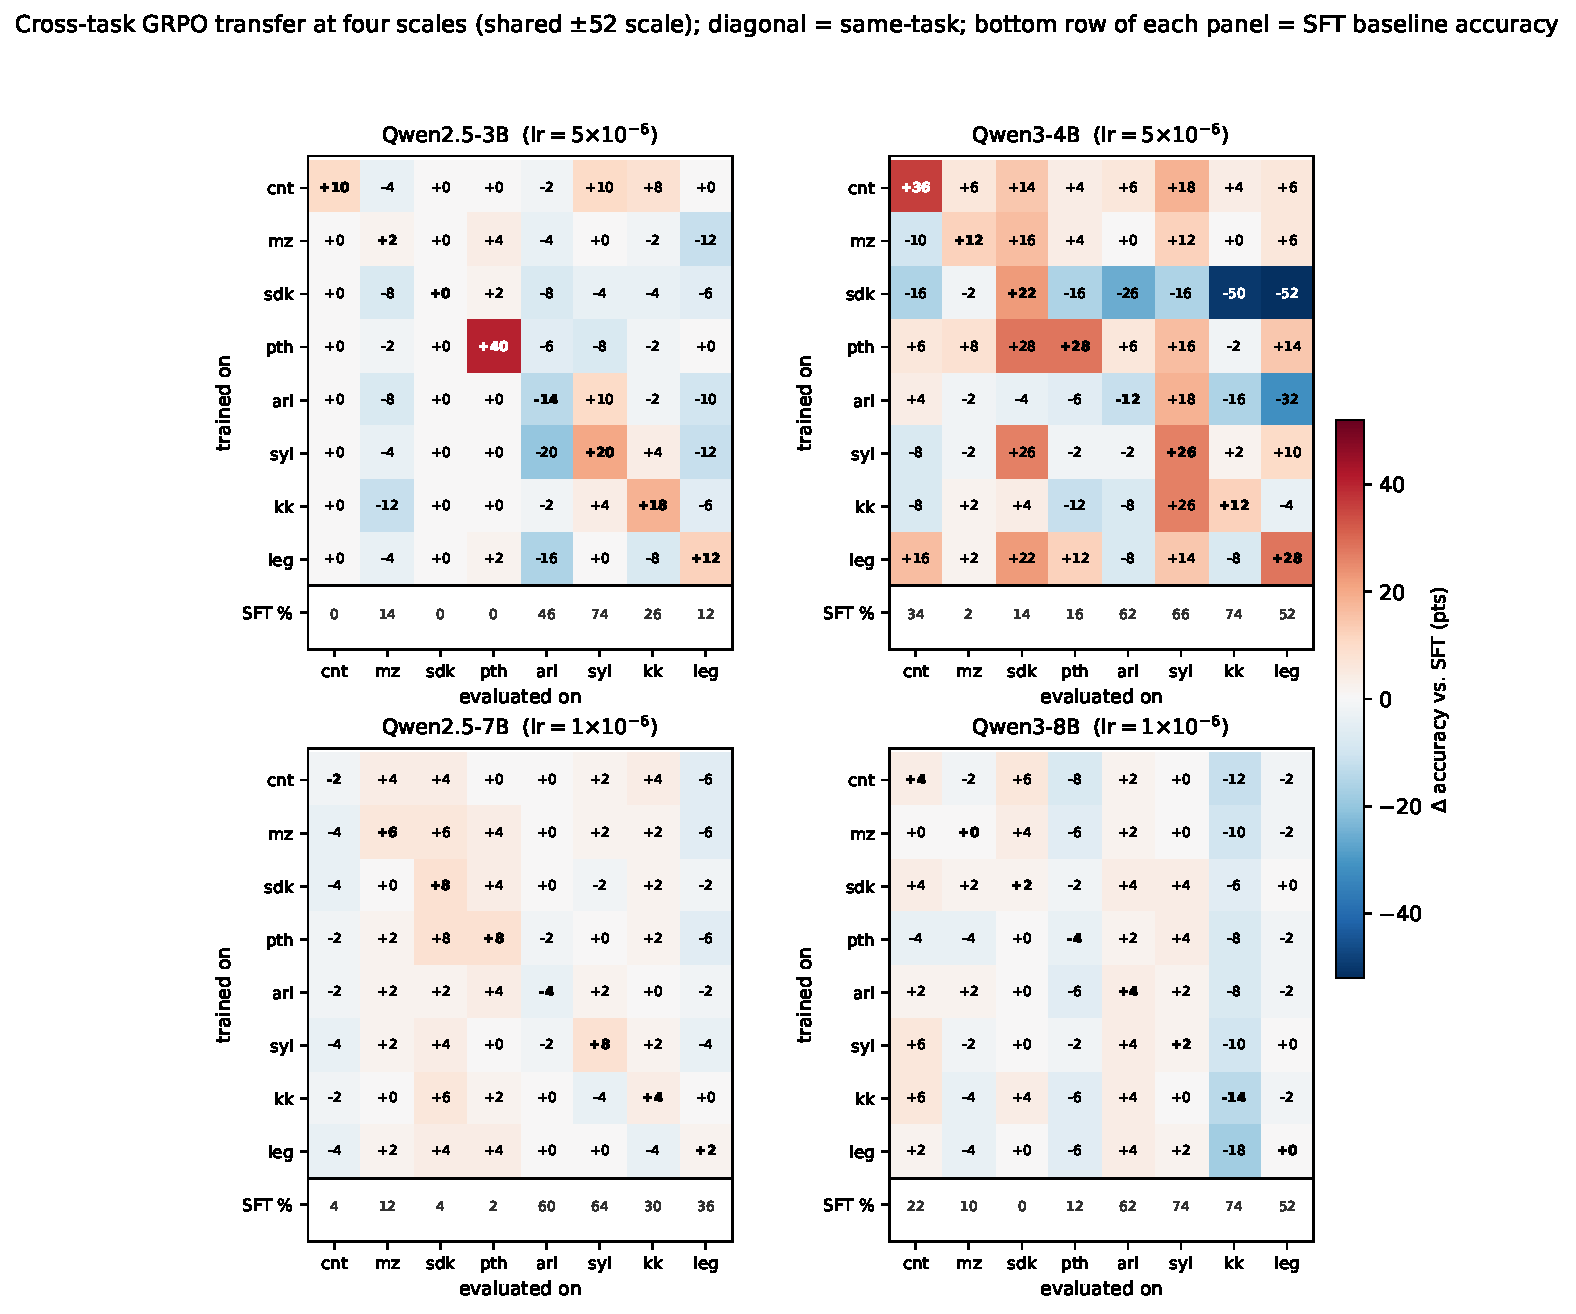
\includegraphics[width=\textwidth]{fig_p1_transfer.pdf}
\caption{\textbf{Cross-task GRPO transfer at all four scales}, on a shared $\pm52$ color scale.
Rows are the training task, columns the evaluation task; cells are $\Delta$ accuracy vs.\ the SFT
baseline (red $=$ gain, blue $=$ loss); the bold diagonal is same-task; the bottom row of each panel
gives the absolute SFT baseline accuracy per task. \emph{Top row} (3B, 4B) uses the aggressive
$\mathrm{lr}{=}5\!\times\!10^{-6}$: the catastrophic 4B \texttt{mini\_sudoku} row ($-50$, $-52$) and
the asymmetric search$\rightarrow$logic / logic$\rightarrow$arithmetic structure are visible at a
glance. \emph{Bottom row} (7B, 8B) uses the gentle $\mathrm{lr}{=}1\!\times\!10^{-6}$ (v2): on the
same scale the entire matrix flattens to within a few points (no cell exceeds $\pm18$), eliminating
both the catastrophic harms and the large gains seen above. The lone systematic exception is the
negative \texttt{kk} column at 8B (GRPO on any task degrades its fragile $74\%$
\texttt{knights\_knaves} baseline).}
\label{fig:p1heat}
\end{figure}

\paragraph{GRPO is not a universal improver.} The headline result is that GRPO is not free
improvement: it helps on some tasks, hurts on others, and across all four matrices it degrades
$36\%$ of (train, eval) task pairs. The damage can be catastrophic and crosses unrelated skills,
training on the constraint-satisfaction task \texttt{mini\_sudoku} at 4B costs $-52$ pts on
\texttt{leg\_counting} and $-50$ on \texttt{knights\_knaves}. GRPO can even hurt the very task it
was trained on: \texttt{basic\_arithmetic} degrades on \emph{itself} at every scale ($-14$ at 3B,
$-12$ at 4B, $-30$ at 7B). Its binary reward rewards short final answers and induces a
\emph{reasoning compression} that skips the intermediate steps multi-digit arithmetic needs, so the
verbose chain-of-thought learned during SFT is a better strategy than anything GRPO discovers.
Large gains coexist with all of this (\texttt{countdown} reaches $+60$ at 7B), but the net effect
is task- and scale-dependent, not a uniform lift.

\paragraph{What consistently helps, what stays inert.} Three tasks improve at \emph{every} scale
and share a common trait: they have clear, learnable reasoning structure that GRPO can sharpen
without needing novel computation. \texttt{syllogism} gains $+18$--$+26$, \texttt{shortest\_path}
$+28$--$+40$, and \texttt{countdown} scales with model size
($+10\!\rightarrow\!+36\!\rightarrow\!+60\!\rightarrow\!+50$ for 3B/4B/7B/8B). At the other extreme,
\texttt{caesar\_cipher} and \texttt{cryptarithm} sit at $0\%$ baseline \emph{and} $0\%$ after GRPO
at all scales: their reward is too sparse (a single wrong character fails the whole answer) to give
any learning signal. Between these lies a capability threshold: \texttt{mini\_sudoku} is unlearnable
below 4B but reaches $+60$ at 8B, once the model has the capacity to track row, column, and subgrid
constraints simultaneously.

\paragraph{Transfer is asymmetric and structured.} Cross-task transfer is not symmetric.
Search and planning training transfers positively to logic (\texttt{countdown}$\rightarrow$
\texttt{syllogism} is $+10$--$+18$; \texttt{shortest\_path}$\rightarrow$\texttt{syllogism} is $+16$
at 4B), but logic training hurts computation (\texttt{syllogism}$\rightarrow$
\texttt{basic\_arithmetic} is $-20$ at 3B and $-46$ at 7B). \texttt{shortest\_path} is the best
all-rounder, lifting $6$ of $9$ other tasks at 4B (up to $+28$ on \texttt{mini\_sudoku}), whereas
training on \texttt{mini\_sudoku} overspecializes the model and is the most destructive to others.
This directional structure is what makes curriculum order matter for multi-task RLVR.

\paragraph{Baselines are strong, and learning rate dominates scale.} SFT alone already reaches
$62$--$78\%$ on arithmetic and syllogism, so GRPO's room to improve over SFT is smaller than is
commonly assumed, and its room to \emph{damage} a strong baseline is correspondingly larger.
On top of this, the learning rate is the dominant hyperparameter. Re-running 7B/8B at the gentle
$\mathrm{lr}{=}1\!\times\!10^{-6}$ (16 generations) collapses both gains and harms: the worst 7B
same-task drop shrinks from $-30$ to $-4$ and the largest gain from $+60$ to $+8$, flattening the
entire matrix to within $\pm18$ pts (Figure~\ref{fig:p1heat} bottom row, Appendix~\ref{app:p1}). The
difference between $5\!\times\!10^{-6}$ and $1\!\times\!10^{-6}$ exceeds the difference between model
sizes; the optimal LR sits between, high enough to learn but low enough to avoid forgetting. These
findings motivate the rest of the paper: \emph{when} does GRPO help (\S\ref{sec:phase2}),
\emph{what} does it change (\S\ref{sec:phase3}), and can those changes be \emph{composed}
(\S\ref{sec:phase4})?

% =====================================================================
\section{Atomic Readiness and the Curriculum Decision}
\label{sec:phase2}
% =====================================================================
The transfer matrix (\S\ref{sec:phase1}) showed that single-task GRPO does not uniformly help,
and that on some tasks it actively destroys a working model (\texttt{maze} collapses to $1\%$).
We now ask \emph{when} GRPO will help, and turn the answer into a cheap pre-training diagnostic.

\paragraph{Why decompose into atoms.} Our starting hypothesis is about capability, not
optimization. A hard reasoning task sits above the small model's current capability frontier: the
model cannot reliably perform even the sub-steps the task is built from, so when we run GRPO
directly on the full task it almost never stumbles onto a correct trajectory. Every sampled
completion then earns near-zero verifiable reward, the group-relative advantage GRPO learns from
is empty, and there is simply nothing to reinforce. Training the full task harder cannot fix this.
The alternative is to \emph{grow the capability up to the task}: decompose it into easier atomic
sub-skills that are already within reach (or nearly so), train those first to extend what the
model can do, and only then expect the full task to become reachable. Under this view atoms are a
curriculum that raises the model's floor until the full-task reward is no longer sparse, giving us
a path to capabilities that direct training cannot reach.

\paragraph{A three-layer taxonomy.} To make ``sub-skill'' precise we decompose any reasoning task
into three layers (Table~\ref{tab:taxonomy}): \textbf{L1 (grounding)} reads the input
representation, \textbf{L2 (local reasoning)} performs a single inference step over grounded
elements, and \textbf{L3 (global planning)} is the multi-step composition that \emph{is} the full
task. L1 and L2 are the sub-skills we can author cheap atoms for and train in isolation; L3 is
what full-task GRPO has to supply. The hypothesis above becomes concrete: when a model cannot do
L1/L2, full-task GRPO has no foothold and thrashes on sparse reward, and an atomic curriculum that
trains the missing layer should help.

\begin{table}[t]
\centering\small
\caption{\textbf{The three-layer task taxonomy, with example atoms.} L1 and L2 are short,
programmatically verifiable Q\&A atoms we author and train directly; L3 is the full task that only
end-to-end GRPO trains. Examples are drawn from \texttt{maze}, \texttt{basic\_arithmetic}, and
\texttt{syllogism}.}
\label{tab:taxonomy}
\begin{tabular}{@{}llp{7.4cm}@{}}
\toprule
Layer & What it tests & Representative atoms (task)\\
\midrule
\textbf{L1} grounding & parse the input &
``What symbol is at row 3, column 5?'' (\texttt{maze}); ``List all numbers in $-66 - -51$''
(\texttt{arithmetic}); ``Which premise contains the word `all'?'' (\texttt{syllogism})\\
\addlinespace
\textbf{L2} local reasoning & one inference step &
``Is moving east from cell $(3,5)$ legal?'' (\texttt{maze}); ``Evaluate $-(52 + -20 + -66)$''
(\texttt{arithmetic}); ``If A$\to$B and A holds, what follows?'' (\texttt{syllogism})\\
\addlinespace
\textbf{L3} global planning & multi-step composition &
give the shortest path from start to goal (\texttt{maze}); evaluate the full multi-operator
expression under order-of-operations (\texttt{arithmetic}); decide whether the syllogism is valid
(\texttt{syllogism})\\
\bottomrule
\end{tabular}
\end{table}

\paragraph{The Atomic Readiness Score.} For each task we hand-author 6--14 atomic Q\&A
\emph{templates} (4--8 L1, 3--6 L2), each a deterministic function of a \texttt{reasoning-gym}
sample with a programmatically verifiable answer. ARS is a pure inference probe: zero-shot the
$\Wsft$ base on 50 samples/atom, extract the last \texttt{<answer>}, score with a
\emph{lenient} type-aware verifier, and average. We report $\mathrm{L1\_avg}$ (grounding floor),
$\mathrm{L2\_avg}$ (local-reasoning floor), and $\mathrm{ARS}$ (overall). The full 7-task probe
costs $\approx$1 GPU-hour. We then compare three matched-compute RLVR regimes:
\textbf{Direct-RLVR} (300 full-task steps), \textbf{Atomic-Only} (100 L1 $\rightarrow$ 100 L2,
zero-shot transfer to the full task), and \textbf{Atomic-Warm} (L1 $\rightarrow$ L2 $\rightarrow$
full).

\begin{table}[t]
\centering\small
\caption{\textbf{ARS predicts the optimal RLVR regime on 6/7 tasks.} Accuracies are full-task
eval. Bold $=$ best regime. ARS bands: high ($>60\%$), medium ($40$--$60\%$), low ($<25\%$).}
\label{tab:p2}
\begin{tabular}{lrrrrrl}
\toprule
Task & ARS & Base & Direct & Atomic-Only & Atomic-Warm & ARS reading\\
\midrule
syllogism        & 74\%   & 79.5 & 96.5 & 81.0 & \textbf{97.0} & high $\to$ GRPO works \cmark\\
knights\_knaves  & 62.5\% & 78.0 & \textbf{97.5} & 79.0 & 95.0 & high $\to$ GRPO works \cmark\\
basic\_arithmetic& 66\%   & 72.0 & 32.0 & \textbf{78.0} & 70.0 & high, but GRPO destructive \cmark\\
countdown        & 56\%   & 26.0 & \textbf{$\sim$70} & 24.0 & 26.0 & medium, L3 bottleneck \cmark\\
maze             & 20.7\% & 21.5 & 1.0  & \textbf{41.0} & 38.5 & low $\to$ atoms essential \cmark\\
shortest\_path   & 14\%   & 10.0 & 44.0 & 12.0 & \textbf{46.0} & low $\to$ atoms help \cmark\\
mini\_sudoku     & 19.8\% & 4.0  & \textbf{25.5} & 17.0 & 24.0 & low, but GRPO wins \xmark\\
\bottomrule
\end{tabular}
\end{table}

\paragraph{Main finding.} ARS alone selects the optimal RLVR regime on 6 of 7 tasks
(Table~\ref{tab:p2}, Figure~\ref{fig:p2}): the band a task falls in (high $>60\%$, medium
$40$--$60\%$, low $<25\%$) tells us \emph{in advance} whether to train the full task directly or to
build an atomic curriculum first. We read the three bands in turn.

\paragraph{Where the curriculum works, and why.} The clearest wins are the low-ARS tasks, exactly
the regime our capability-frontier hypothesis predicts. \texttt{maze} (ARS $20.7\%$) cannot even
locate start and goal, so Direct-RLVR collapses to $1\%$, \emph{below} its $21.5\%$ base: GRPO
never samples a correct trajectory and so has nothing to reinforce. Teaching the grounding atoms
first lifts it to $41\%$ with no full-task training at all. \texttt{shortest\_path} (ARS $14\%$) is
the same story, atoms take it from $10\%$ to $46\%$ ($55.5\%$ with the refinements of
Appendix~\ref{app:sp}) where Direct-RLVR stalls at $44\%$. The mechanism is the one we hypothesized:
when the L1/L2 floor is at zero the full-task reward is too sparse for GRPO to climb, and the only
way forward is to \emph{raise the floor} by training the missing sub-skills until the task comes
within reach. The high-ARS tasks confirm the converse half of the same prediction: \texttt{syllogism}
and \texttt{knights\_knaves} already clear both floors, so Direct-RLVR reaches $\approx 97\%$ and
atoms add almost nothing, ARS correctly tells us \emph{not} to spend the extra compute.

\paragraph{The middle case.} Medium-ARS \texttt{countdown} ($56\%$) is the instructive in-between.
Its floors are split (weak L1 number-handling, strong L2 arithmetic), but the real bottleneck is
neither: it is the L3 search for a combination that hits the target, which no atom teaches.
Accordingly both atomic regimes stay at base ($24$--$26\%$) while only Direct-RLVR moves it
($\sim$$70\%$). This is consistent with the hypothesis rather than a failure of it: atoms help only
when the missing capability lives at L1 or L2, and when the gap is purely L3 planning the full task
is the only thing that can supply it.

\paragraph{Where it does not work, and why.} The lone misprediction is \texttt{mini\_sudoku}: low
ARS ($19.8\%$) yet Direct-RLVR ($25.5\%$) beats both atomic regimes. This is the honest boundary of
the method, not a counterexample to the mechanism. Sudoku's true bottleneck is multi-cell constraint
propagation, a holistic L2--L3 operation, but our single-hop atoms only probe isolated cell reads, so
the ARS we measured is uncorrelated with the actual difficulty and the curriculum ends up training
the wrong skill. The lesson is a clean one: \emph{ARS is only as predictive as the atoms are well
chosen}; when the atoms miss the task's real bottleneck, so does the score.

\begin{figure}[t]
\centering
\begin{subfigure}{0.49\textwidth}
  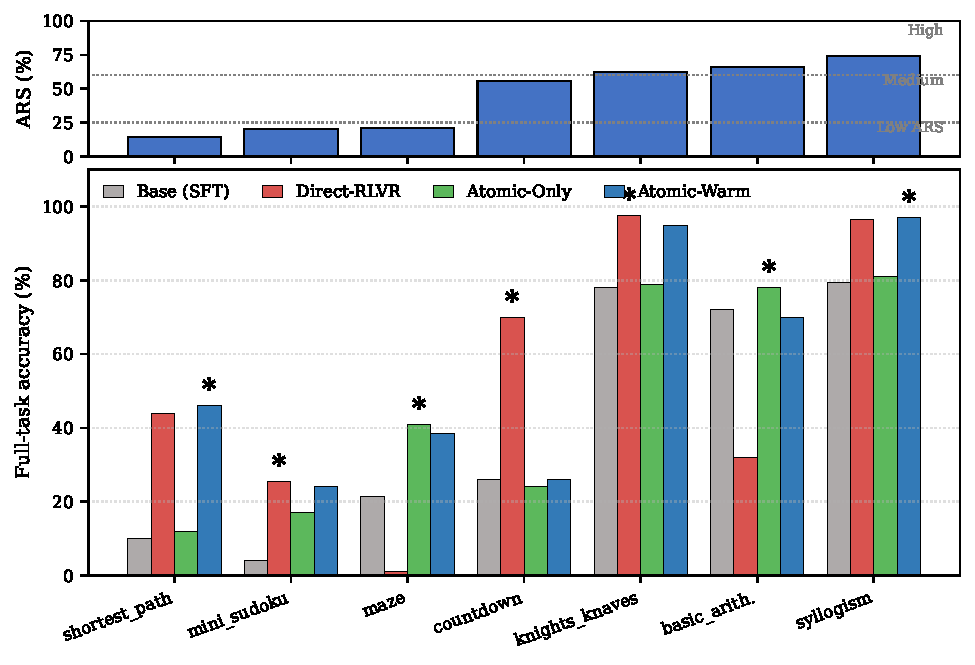
\includegraphics[width=\textwidth]{fig4_1_ars_regime_comparison.pdf}
  \caption{Best regime by ARS band.}
\end{subfigure}\hfill
\begin{subfigure}{0.49\textwidth}
  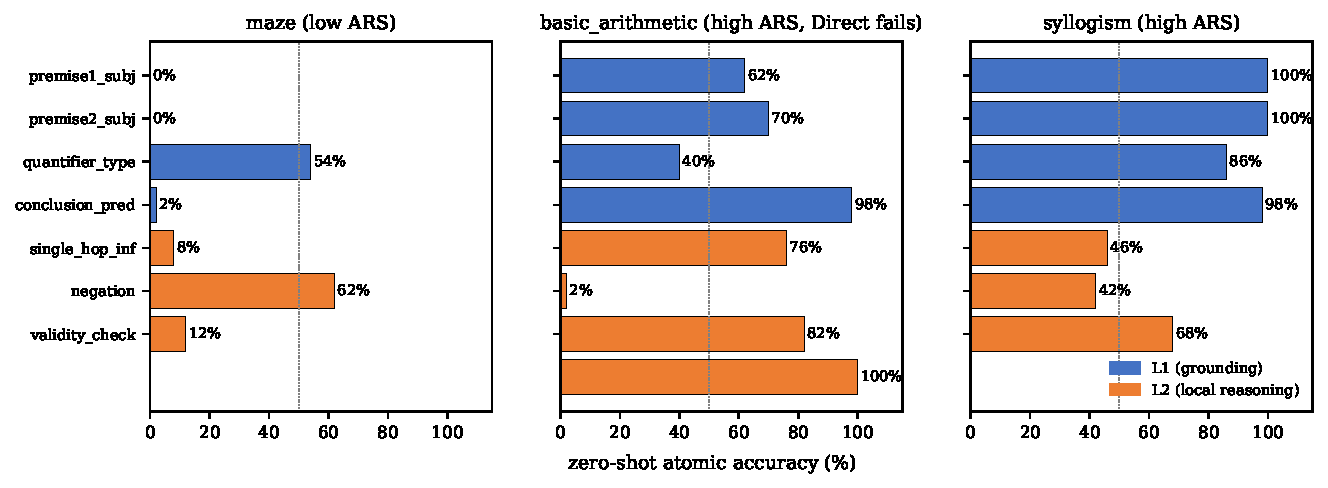
\includegraphics[width=\textwidth]{fig4_2_atom_breakdown.pdf}
  \caption{L1/L2 atom accuracies per task.}
\end{subfigure}
\caption{\textbf{Atomic readiness.} (a) ARS partitions tasks into regimes; (b) the L1/L2
decomposition exposes which floor (grounding vs.\ local reasoning) is missing.}
\label{fig:p2}
\end{figure}

\paragraph{The arithmetic anomaly and reasoning compression.} \texttt{basic\_arithmetic} breaks
the naive ``high ARS $\Rightarrow$ GRPO works'' rule: despite $\mathrm{ARS}{=}66\%$,
Direct-RLVR collapses it to $32\%$. The cause is reasoning compression: GRPO shortens
outputs (Atomic-Only $386$ chars $\rightarrow$ Atomic-Warm $234$ chars), skipping the
order-of-operations steps (the \texttt{order\_of\_operations} atom sits at just $2\%$ on the base
model, the single weakest atom in the arithmetic decomposition). Generation logs at 8B make the
mechanism visible directly: the SFT model writes out each step (``Subtracting a negative is like
adding the positive$\ldots$'', $\approx 200$ chars/response), whereas the GRPO model collapses to a
terse ``$-66 - -51 = -15$'' ($\approx 70$ chars). The short form is correct on one-step problems
but fails on multi-step expressions like \texttt{-3241 - 2720 - 9730 + 6743 + 1933} where the
intermediate values must be carried. ARS measures grounding readiness, not GRPO's reward dynamics;
tasks with long obligatory reasoning chains can be harmed even at high ARS.

\paragraph{Craft lessons from pushing the hardest task.} \texttt{shortest\_path} is the lowest-ARS
task in the suite (ARS $14\%$, base $10\%$), so we used it as a stress test for how far an atomic
curriculum can be pushed. Across 16 controlled training conditions (Figure~\ref{fig:sp}; full table
in Appendix~\ref{app:sp}) we took it from $10\%$ to $55.5\%$, a $5.5\times$ improvement and $+11.5$
points over plain Direct-RLVR. The conditions that helped, and the ones that backfired, distill into
four reusable lessons for RLVR on hard tasks.

\begin{itemize}\itemsep3pt
\item \textbf{Match the atom's answer shape to the task.} Short yes/no grounding atoms train the
model to emit one-token answers, the same reasoning compression we saw on arithmetic; transferred
to a task that needs a written-out path this collapses to $12\%$, \emph{below} the base. Replacing
them with multi-step path-tracing atoms, whose answers are themselves short trajectories, removes
the compression and lifts the otherwise-identical pipeline to $51.5\%$.
\item \textbf{Prefer one hard jump over a gentle ramp.} A progressive curriculum
($3{\times}3\to4{\times}4\to$ full grid) lets the model over-fit easy instances and plateau
($27.5\%$); a single hard transition straight from atoms to full-size grids forces it to generalize
and does markedly better.
\item \textbf{Keep the reward binary.} Partial-credit rewards feel helpful but hurt GRPO ($35.5\%$,
and $24\%$ when stacked with a progressive ramp). GRPO learns from the \emph{variance} of rewards
within a sampled group, so a smooth reward that gives every rollout a similar middling score
flattens that variance and leaves the group-relative advantage with almost nothing to push on. The
sparse, verifiable $0/1$ reward gives the sharpest learning signal.
\item \textbf{RFT-Base spends the whole budget on the real task.} The strongest recipe ($55.5\%$)
generates verified-correct traces from an already-trained model, supervised-fine-tunes the
\emph{base} model on them, and only then runs GRPO. Starting from a clean but already-capable
initialization lets the entire GRPO step budget go to the full task, rather than being split between
atoms and task.
\end{itemize}

\noindent A failure analysis of the $51.5\%$ model (Appendix~\ref{app:sp}) shows the residual errors
are dominated by a ``give-up reflex'' (declaring no path exists when one does); removing that single
behavior alone would reach $68\%$, pointing to where the next gains lie. None of these regimes harms
general ability: an MMLU-math evaluation across 48 checkpoints spanning every part of the study finds
no catastrophic forgetting (within $\pm 3\%$ of base; Appendix~\ref{app:mmlu}).

\begin{figure}[t]
\centering
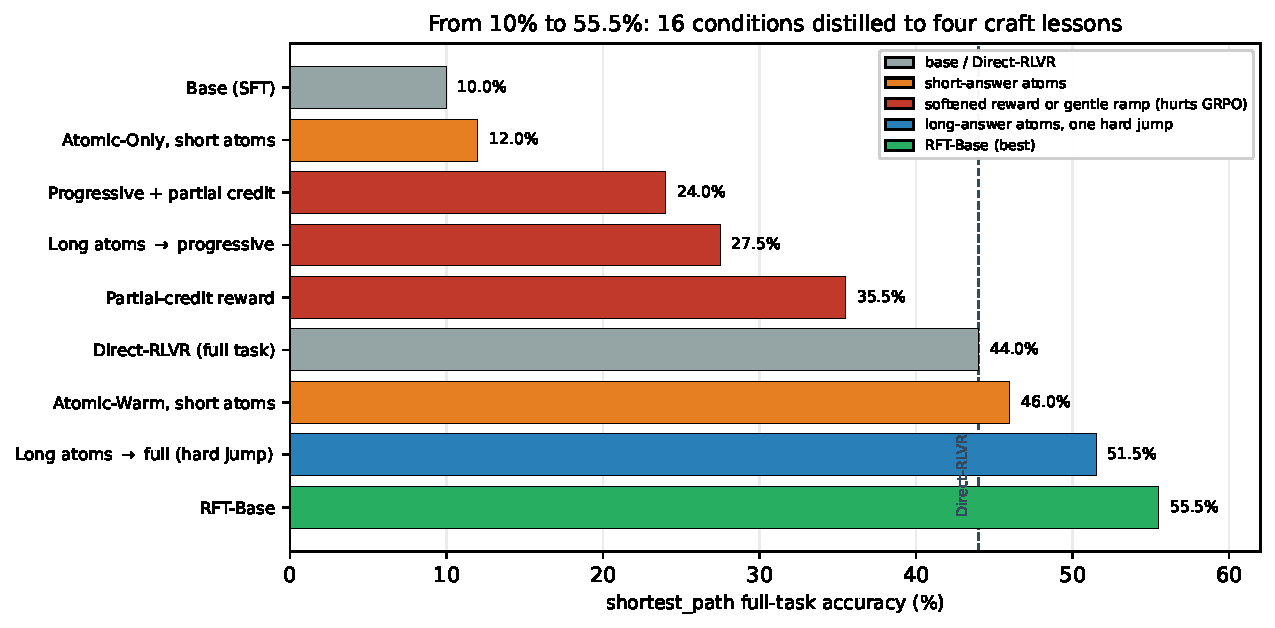
\includegraphics[width=0.86\textwidth]{fig_p2_sp.pdf}
\caption{\textbf{Climbing the hardest task.} Sixteen training conditions take \texttt{shortest\_path}
from a $10\%$ base to $55.5\%$. Bars are sorted by accuracy and colored by lesson category; the
dashed line marks plain Direct-RLVR ($44\%$), the bar to beat. Softened rewards and gentle
difficulty ramps (red) fall \emph{below} Direct-RLVR, short-answer atoms (orange) compress the
output, and the wins come from long-answer atoms with one hard transition (blue) and RFT-Base
(green).}
\label{fig:sp}
\end{figure}

\paragraph{Looking ahead: from growing one skill to composing many.} The atomic curriculum shows
how to bring a \emph{single} hard skill within a small model's reach by raising its capability
floor. The rest of the paper asks the complementary question: once several skills have been trained
separately, can they be \emph{combined} into one model without retraining, simply by adding their
GRPO task vectors? We first characterize what GRPO does to the weights (\S\ref{sec:phase3}) and find
a geometry that looks ideal for composition, each task vector is tiny ($0.06$--$0.12\%$ of the
weights), nearly orthogonal to the base, and nearly orthogonal to other tasks' vectors. We then test
merging head-on (\S\ref{sec:phase4}) and reach a split verdict that previews the paper's central
tension: \emph{construction is easy} (summing two task vectors yields a working multi-skill model,
and one geometry-derived edit, dropping the never-moving \texttt{mlp.down\_proj} block, is safe on
$40/48$ cells), but \emph{prediction is hard} (no cheap probe says in advance which pairs merge
cleanly; damage ranges from $0.5$ to $64.5$ points at near-identical global statistics). Tellingly,
the readiness logic that works so well in this section does \emph{not} carry over: neither ARS nor
the sequential-transfer matrix of \S\ref{sec:phase1} predicts merge compatibility ($r\approx 0$),
because merging is governed by a few localized per-parameter sign conflicts that every averaged
metric washes out.

% =====================================================================
\section{The Weight-Space Geometry of GRPO}
\label{sec:phase3}
% =====================================================================
Having established \emph{when} GRPO helps (\S\ref{sec:phase1}--\S\ref{sec:phase2}), we now open the
model and ask what it physically does to the weights. For every (model scale, task) pair we form the
\textbf{task vector}
$$\tv \;=\; \Wg - \Wsft$$
per weight matrix, the delta GRPO writes on top of the SFT base, and characterize it
geometrically. We track six quantities, each isolating a distinct way a fine-tuning update can act
on a weight matrix $W$ (with singular value decomposition $W=U\Sigma V^\top$, singular values
$\sigma_1\!\geq\!\sigma_2\!\geq\!\cdots$, and top-$k$ singular vectors $U_k,V_k$). Full definitions,
estimators, and random-matrix baselines are in Appendix~\ref{app:geom}.

\begin{itemize}\itemsep2pt
\item \textbf{Update magnitude} $\|\tv\|_F/\|W\|_F$: how big is the edit relative to the weight it
edits?
\item \textbf{Singular-value shift} $\sigma_i(\Wg)$ vs.\ $\sigma_i(\Wsft)$: does GRPO amplify or
shrink the directions $W$ already uses?
\item \textbf{Effective rank} $\exp\!\big(H(\sigma/\!\sum\sigma)\big)$ (entropy of the singular-value
distribution): does GRPO concentrate or spread out $W$'s information?
\item \textbf{Subspace projection} $\rho_k(\tv)=\|U_kU_k^\top\,\tv\,V_kV_k^\top\|_F^2/\|\tv\|_F^2$:
what fraction of the update lands inside $W$'s top-$k$ directions, versus the random baseline
$(k/r)^2$?
\item \textbf{Basis rotation} $\arccos\sigma_i\!\big(U_{\mathrm{SFT}}^\top U_{\mathrm{GRPO}}\big)$
(principal angles): even with the $\sigma_i$ fixed, do the singular \emph{directions} swivel?
\item \textbf{Depth signature} $\mathrm{depth}[\ell]=\sum_{\text{matrices at block }\ell}\|\tv\|_F$:
where along the network's depth does a task concentrate its changes?
\end{itemize}

The picture splits cleanly in two. \emph{How} GRPO edits a weight matrix is near-universal across
tasks, scales, and model families; \emph{where} it edits (which depths, and in which direction) is task-specific. We take the two halves in turn.

\subsection{How GRPO edits: a universal, spectrum-preserving, rotation-localized signature}

Every quantity in this subsection is computed \emph{per (task, weight-matrix)} and reported as a mean
over the tasks trained at each scale, grouped by layer type. The ``universal'' label is itself an
empirical claim about the across-task spread: it is negligible (the per-layer-type rotation varies by
$<0.1\dg$ across tasks, and the $\pm$ figures below are across-task standard deviations; the full
per-metric across-task spread is in Appendix~\ref{app:geom}, Table~\ref{tab:p3-spread}), so the
task-averaged numbers and the per-task numbers coincide, which is exactly why this half is universal
and the ``where'' half below is not.

\paragraph{GRPO preserves the spectrum.} The singular values $\sigma_i$ of a weight matrix are the
gains it applies along its principal directions; the largest, $\sigma_1$ (the spectral norm), is
the biggest factor by which $W$ can stretch any input vector, and the full ordered set
$\sigma_1\!\geq\!\sigma_2\!\geq\!\cdots$ is the natural ``size and shape'' descriptor of a linear
map. We compare these gains before and after training (Fig.~\ref{fig:p3a}a). On the most-changed
layers the spectral-norm ratio $\sigma_1(\Wg)/\sigma_1(\Wsft)$ is $1.000\pm0.002$, the effective
rank moves by less than $0.01$, and a full-SVD sweep over twelve representative layers finds that
\emph{every} singular value shifts by less than $0.1\%$, at or below the bfloat16 rounding floor.
\textbf{These statements hold at all four scales (3B, 4B, 7B, 8B) and across both model families}
(Qwen2.5 at 3B/7B, Qwen3 at 4B/8B): the spectrum is preserved everywhere we looked. GRPO therefore
neither amplifies, dampens, nor re-ranks the directions $W$ already uses. Yet behavior demonstrably
changes (\S\ref{sec:phase1}--\S\ref{sec:phase2}), so the entire learned change must live in
directions that the SVD of $W$ alone cannot see. The next two measurements locate them.

\paragraph{The update writes into the directions $W$ was \emph{not} using.} Intuition first.
Picture $W$ as a machine that listens loudly to a handful of input directions and mostly ignores
the rest. Its top singular directions are the loud ones. GRPO's update $\tv$ could do one of two
things: (i) push harder along those same loud directions, merely turning the existing knobs up or
down, or (ii) write into the quiet, ignored directions, adding genuinely new behavior. The
subspace-projection ratio $\rho_k(\tv)$ measures exactly this: of all the ``energy'' in $\tv$,
what fraction lands inside $W$'s top-$k$ directions? A purely random update would, by chance, land a
fraction $(k/r)^2$ of its energy there; that is our dashed null baseline. We find $\rho_k$ sitting
\emph{at or below} that chance line at 4B and 8B (Fig.~\ref{fig:p3a}b): GRPO is doing (ii), not (i).
It edits the under-used subspace and leaves the dominant machinery alone, which is precisely
\emph{why} the spectrum (the gains of that dominant machinery) does not move. The effect even
\emph{strengthens} with scale: the share of $\tv$ lying in $W$'s top-100 directions falls from
$0.34\%$ at 3B to $0.04\%$ at 7B, so larger models confine GRPO to an ever-thinner, ever-more-
orthogonal sliver of weight space. This is the low-intrinsic-dimensionality picture of fine-tuning
\citep{aghajanyan2021intrinsic,hu2022lora}, which GRPO exhibits even more sharply than supervised
fine-tuning.

\paragraph{The update has its own low-rank structure, and a clean zero control.} The spectrum of
$W$ is pinned, but $\tv$ itself is not spectrally trivial: its \emph{own} singular values decay
$2.5\dg$--$4.2\times$ across the top ten (4B, averaged over \texttt{mlp.down\_proj} layers), so each
task's update concentrates in a handful of preferred directions rather than spreading
isotropically. The leading $\sigma_1(\tv)$ scales with how much a task moves the model: largest for
\texttt{maze} ($0.018$) and \texttt{knights\_knaves} ($0.017$), smallest for the
barely-learnable \texttt{mini\_sudoku} ($0.006$). At the bottom end sits a clean control:
\texttt{cryptarithm} never earns a reward at 4B, so its task vector is \emph{exactly} zero at
every layer ($\|\tv\|_F=0.000$); the geometry pipeline therefore measures learning, not numerical
noise. Per-task $\|\tv\|_F$ and $\sigma(\tv)$ values are tabulated in Appendix~\ref{app:geom}.

\begin{figure}[t]
\centering
\begin{subfigure}{0.49\textwidth}
  \centering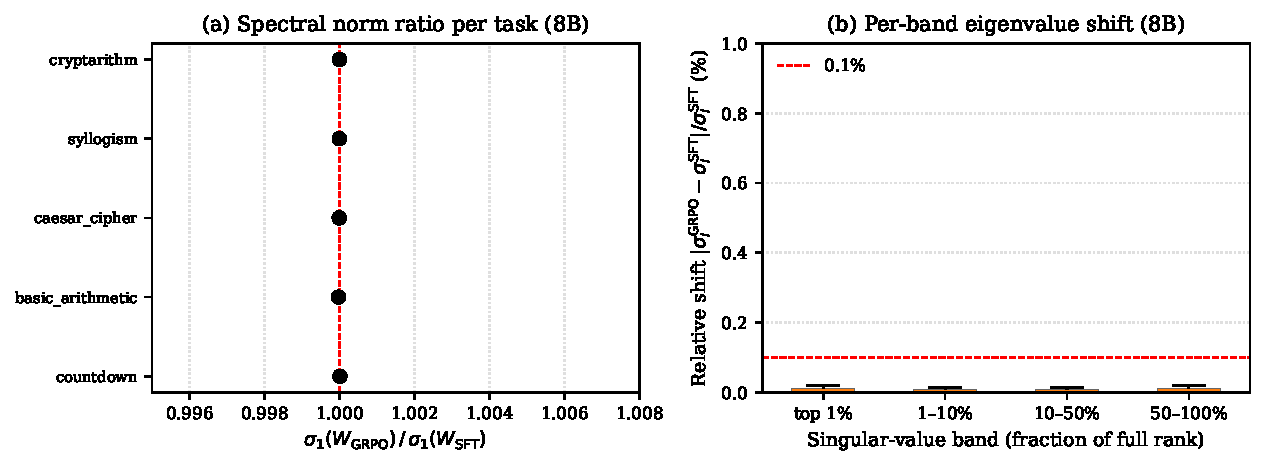
\includegraphics[width=\textwidth]{fig5_1_spectrum_preserved.pdf}
  \caption{Spectrum preserved: $\sigma_i(\Wg)\approx\sigma_i(\Wsft)$.}
\end{subfigure}\hfill
\begin{subfigure}{0.49\textwidth}
  \centering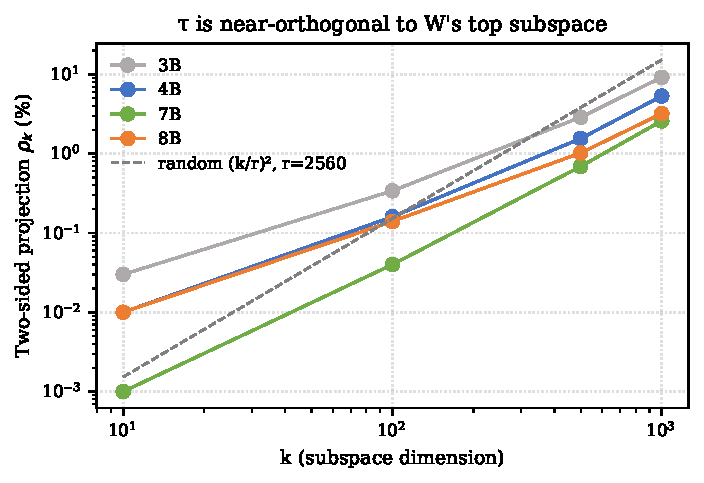
\includegraphics[width=\textwidth]{fig5_2_tau_orthogonal.pdf}
  \caption{$\tv$ projection onto $W$'s top-$k$ tracks the random baseline $(k/r)^2$.}
\end{subfigure}

\vspace{1.5ex}
\begin{subfigure}{0.62\textwidth}
  \centering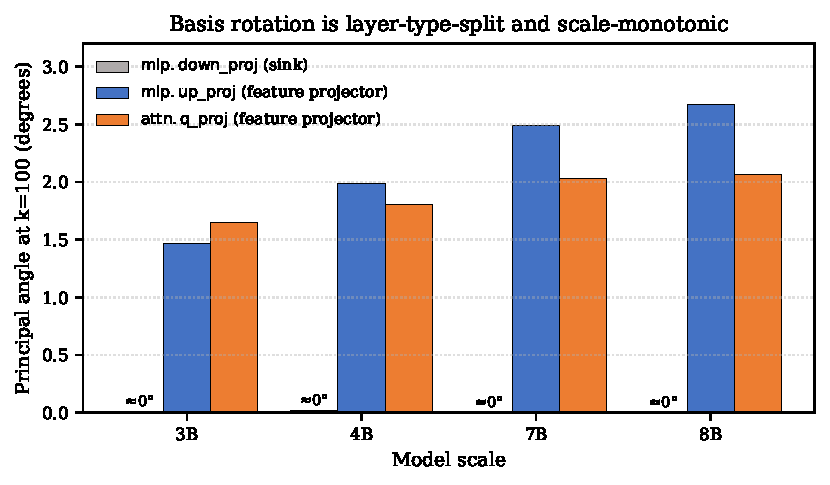
\includegraphics[width=\textwidth]{fig5_3_layer_type_rotation.pdf}
  \caption{Basis rotation by layer type and scale: \texttt{down\_proj} frozen, feature
  projectors rotate $1.5\dg$--$2.7\dg$.}
\end{subfigure}
\caption{\textbf{The universal ``how'' of GRPO.} The update preserves $W$'s spectrum (a), lives in
the directions $W$ was not using (b), and rotates feature-projector bases while leaving the MLP
sink \texttt{mlp.down\_proj} frozen (c). Every panel holds across 3B/4B/7B/8B and both Qwen
families.}
\label{fig:p3a}
\end{figure}

\paragraph{The frozen-sink invariant.} The spectrum is pinned, but the singular \emph{vectors}, the directions themselves, can still swivel without changing any $\sigma_i$. We quantify that
swivel as the principal angle between $\Wsft$'s and $\Wg$'s top-100 singular subspaces ($0\dg$ =
identical directions, $90\dg$ = fully reoriented). Averaged over all layers it is a mild
$1\dg$--$3\dg$, but breaking it out by layer type (Table~\ref{tab:p3-rot}, Fig.~\ref{fig:p3a}c; the
per-task de-aggregation behind these averages is in Appendix~\ref{app:geom},
Table~\ref{tab:p3-pertask-rot})
exposes the cleanest invariant in the study: \texttt{mlp.down\_proj} rotates $0.00\dg$--$0.02\dg$, effectively \emph{frozen}, at every scale and in both families, while the feature projectors
\texttt{mlp.up\_proj} and \texttt{attn.q\_proj} rotate $1.5\dg$--$2.7\dg$, growing monotonically
with model size. The mechanism is intuitive once named. \texttt{down\_proj} and \texttt{attn.o\_proj}
are \emph{sinks}: they sum contributions from many neurons back into the residual stream, so their
dominant directions are pinned by the aggregate statistics of all inputs and resist reorientation.
\texttt{up\_proj} and \texttt{q\_proj} are \emph{feature projectors}: they decide which features to
compute and what to attend to, so they are the natural site for installing task-specific behavior,
and they rotate accordingly. The zero-rotation result is specific to the MLP sink: the attention
sinks are \emph{not} literally frozen, with \texttt{attn.k} rotating $30\dg$--$42\dg$ and
\texttt{attn.\{v,o\}} $50\dg$--$70\dg$ in the merge analysis of \S\ref{sec:phase4}.

\begin{table}[t]
\centering\small
\caption{\textbf{Basis rotation by layer type} (principal angle at $k{=}100$, degrees).
\texttt{mlp.down\_proj} is frozen at every scale; feature projectors rotate, growing with scale.}
\label{tab:p3-rot}
\begin{tabular}{lrrrr}
\toprule
Layer type & 3B & 4B & 7B & 8B\\
\midrule
\texttt{mlp.down\_proj} & $0.01\dg$ & $0.02\dg$ & $0.00\dg$ & $0.00\dg$\\
\texttt{mlp.up\_proj}   & $1.47\dg$ & $1.99\dg$ & $2.49\dg$ & $2.67\dg$\\
\texttt{attn.q\_proj}   & $1.65\dg$ & $1.81\dg$ & $2.03\dg$ & $2.07\dg$\\
\bottomrule
\end{tabular}
\end{table}

\subsection{Where GRPO edits: same rotation budget, different direction and depth}

If every task rotates the feature projectors by the same $\sim$2$\dg$, what makes one task vector
differ from another? Two things: the \emph{direction} of the rotation and its \emph{depth}.

\paragraph{Same budget, different direction.} The rotation \emph{amount} is almost task-independent:
across tasks at a fixed scale it varies by less than $0.1\dg$, as if GRPO spends a fixed ``rotation
budget'' per layer type no matter what it is learning (consistent with the near-uniform
$\|\tv\|_F\!\approx\!0.7$--$1.2$ at 4B reported in \S\ref{sec:phase4}). What differs is \emph{which
way} each task turns. We extract the new directions a task introduces (its \emph{novel subspace}:
the part of $\Wg$'s top-$k$ basis lying outside $\Wsft$'s; defined in Appendix~\ref{app:geom}).
Rotation \emph{direction} is only meaningful relative to another task, so the natural measure is
inherently \emph{pairwise}: the principal angle between \emph{two} tasks' novel subspaces ($0\dg$ =
same new direction, $90\dg$ = perpendicular), which has no single-task analogue. Figure~\ref{fig:p3b}a
reports this angle for all six pairs among the four tasks, layer by layer within each layer type, so
each cell asks ``do tasks $A$ and $B$ rotate this layer the same way?''. Tasks genuinely
diverge: pairwise angles average $24\dg$ on \texttt{mlp.down\_proj} (its tiny novel subspace is the
least task-specific), $39\dg$ on \texttt{mlp.up\_proj}, and $43\dg$ on \texttt{attn.q\_proj}, the
most task-adversarial layer type, where individual layers swing from strongly aligned ($+0.89$
flat cosine) to directly opposing ($-0.90$) depending on the task pair (Fig.~\ref{fig:p3b}a). Those
local oppositions are the microscopic seed of the catastrophic cross-task degradation in
\S\ref{sec:phase1}, and, later, of merge damage.

\paragraph{Different depth.} Tasks also disagree on \emph{where} along the network's depth to write.
A task's depth signature, the profile of $\|\tv\|_F$ across layer indices, is sharply
task-specific (Fig.~\ref{fig:p3b}b). At 8B, \texttt{caesar\_cipher} packs $88\%$ of its change into
the early layers (fitting a token-level substitution task), the arithmetic tasks (\texttt{countdown},
\texttt{basic\_arithmetic}) edit mid-late layers, and the logic tasks cluster in the mid-early band.
These signatures are not fixed: they shift with model scale, and the \emph{direction} of the shift is
itself task- and family-dependent (Fig.~\ref{fig:p3b}c; the full per-task migration for all nine
tasks is in Appendix~\ref{app:geom}, Fig.~\ref{fig:p3pertaskdepth}). Comparing the two scales \emph{within} each
family, which removes the Qwen2.5-vs-Qwen3 confound, every task we track deepens from 3B to 7B in
Qwen2.5, whereas within Qwen3 the movement splits: \texttt{basic\_arithmetic} and
\texttt{shortest\_path} deepen from 4B to 8B, while \texttt{syllogism} and \texttt{caesar\_cipher}
move \emph{shallower} (the latter consolidating $88\%$ of its change into the early layers at 8B).
With only two scales per family this fixes the direction of movement, not a monotonic trend; either
way, an interference or curriculum analysis calibrated on one model will mispredict another.
Finally, depth-profile overlap predicts the sequential-transfer outcomes of \S\ref{sec:phase1}
\emph{better} than whole-model task-vector cosine, which is $<0.1$ for every task pair and explains
only $\sim$10\% of the transfer variance (Pearson $r{=}0.32$): the conflict is local in depth, and a
global average washes it out. The worst transfer in the entire study makes this concrete:
\texttt{mini\_sudoku}$\rightarrow$\texttt{leg\_counting} ($-52$ at 4B) has near-zero global $\tv$
cosine, yet its depth-profile cosine is $0.33$ because \texttt{mini\_sudoku} concentrates its change
in \texttt{L19}--\texttt{21} while \texttt{leg\_counting} relies on \texttt{L12}--\texttt{16} and is
\emph{negatively} loaded at \texttt{L19}--\texttt{21}; training on \texttt{mini\_sudoku} overwrites
exactly the layers \texttt{leg\_counting}'s output stages depend on.

\begin{figure}[t]
\centering
\begin{subfigure}{0.49\textwidth}
  \centering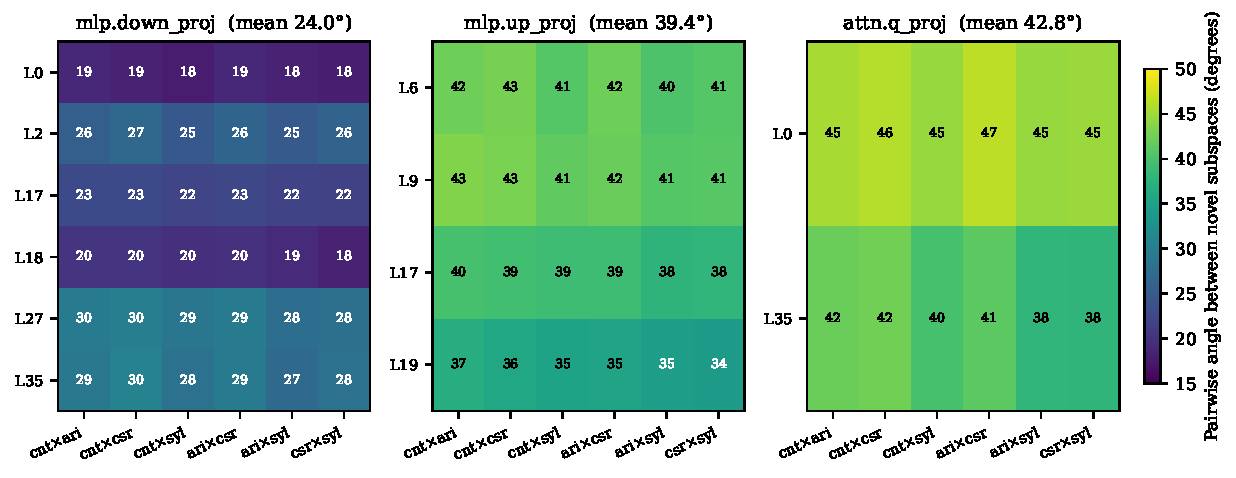
\includegraphics[width=\textwidth]{fig5_4_novel_subspace_angles.pdf}
  \caption{Principal angle between each task \emph{pair}'s novel subspaces (rows = layers within a
  type, columns = the six task pairs). Larger = the two tasks add more divergent new directions:
  $24\dg$--$43\dg$, largest on \texttt{attn.q\_proj}.}
\end{subfigure}\hfill
\begin{subfigure}{0.49\textwidth}
  \centering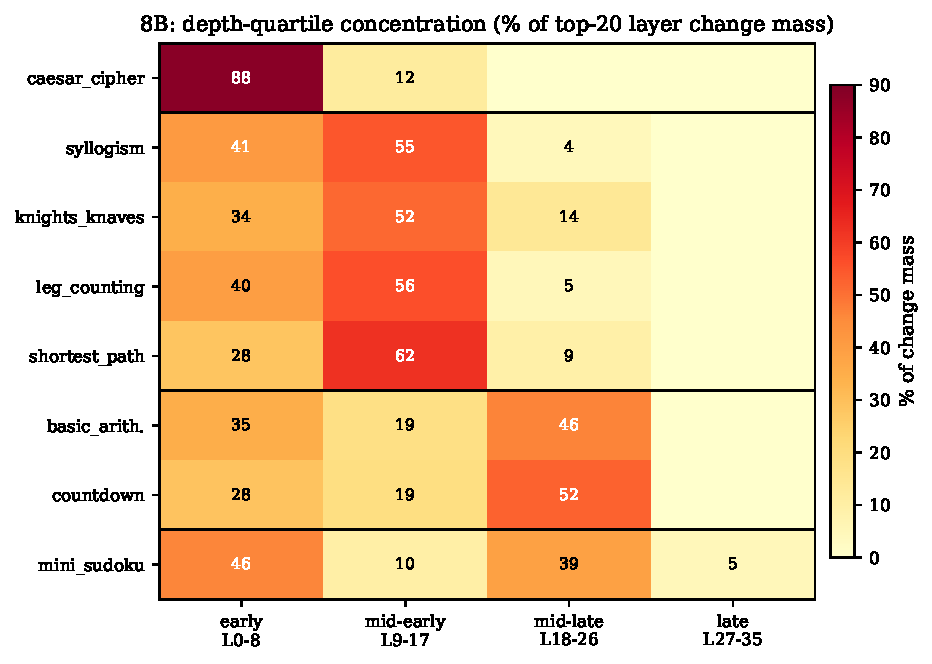
\includegraphics[width=\textwidth]{fig5_5_depth_signatures_8b.pdf}
  \caption{Depth signatures at 8B: each task concentrates change at a different depth.}
\end{subfigure}

\vspace{1.5ex}
\begin{subfigure}{0.62\textwidth}
  \centering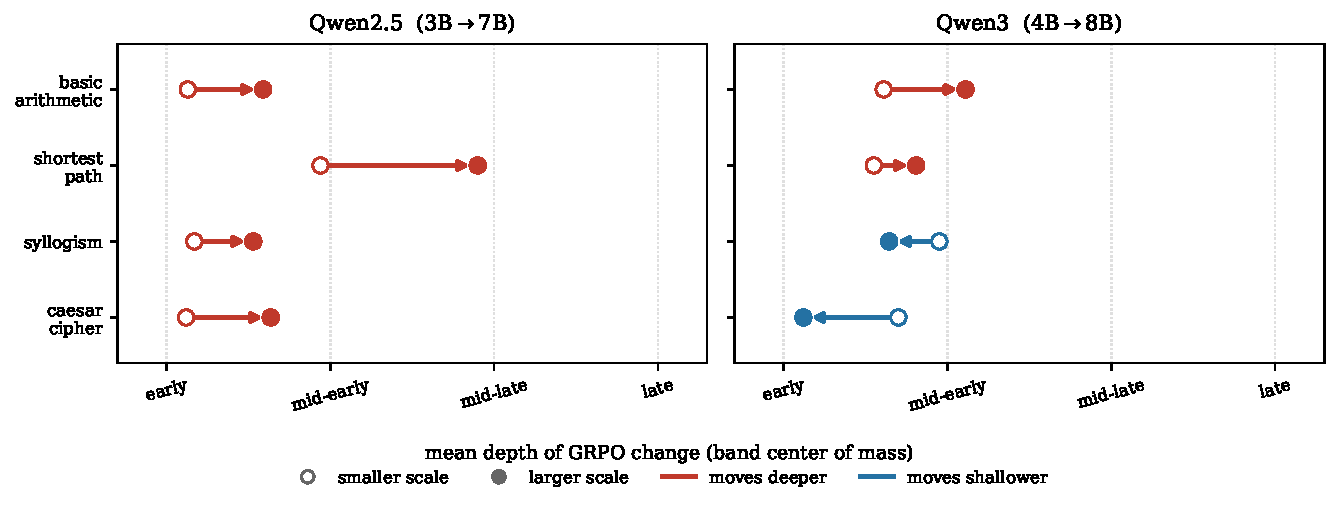
\includegraphics[width=\textwidth]{fig5_6_scale_depth_migration.pdf}
  \caption{Depth migration within each family (mean depth of change, smaller$\to$larger scale).
  Qwen2.5 tasks (3B$\to$7B) all deepen; in Qwen3 (4B$\to$8B) movement splits:
  \texttt{basic\_arithmetic}/\texttt{shortest\_path} deepen, \texttt{syllogism}/\texttt{caesar\_cipher}
  move shallower.}
\end{subfigure}
\caption{\textbf{The task-specific ``where'' of GRPO.} Rotation \emph{magnitude} is task-invariant,
but the \emph{direction} of rotation (a) and the \emph{depth} at which change concentrates (b),
together with how that depth shifts across scale within each model family (c), are all task-specific.}
\label{fig:p3b}
\end{figure}

\subsection{What this geometry implies for merging}

Three of these facts make adding task vectors back onto the base (\emph{task arithmetic})
look theoretically safe. $\tv$ is small relative to $W$ ($0.06\%$--$0.12\%$ in Frobenius norm), it
is near-orthogonal to $W$'s dominant subspace, and different tasks' $\tv$'s are near-orthogonal to
one another (global cosine $0.00$--$0.08$), so summing them should not produce destructive
interference. One fact is even directly actionable: if \texttt{mlp.down\_proj}'s basis never moves,
its $\tv$ contribution may be noise that a merge can safely discard. The next section tests both the
optimistic geometry and this concrete recipe, and finds that the geometry delivers the recipe,
but not the prospective predictability one would hope for.

% =====================================================================
\section{Characterizing Task-Vector Merging}
\label{sec:phase4}
% =====================================================================

\paragraph{Background.} We merge single-task RLVR vectors by task arithmetic
\citep{ilharco2023editing}, $W_{\mathrm{merged}} = \Wsft + s\sum_i \tv_i$, and ask: do RLVR vectors compose into multi-skill
models, and can we predict \emph{which} merges work? We evaluate 19 pairs at 4B (subsets at 3B/8B)
and define \emph{pair damage} as the total per-task accuracy a merge loses relative to the two
single-task sources, $\mathrm{damage}(A,B)=\max(0,\mathrm{acc}_A^{\mathrm{src}}-\mathrm{acc}^{\mathrm{merge}})
+\max(0,\mathrm{acc}_B^{\mathrm{src}}-\mathrm{acc}^{\mathrm{merge}})$. Damage spans $0.5$ to
$64.5$ points across the 19 pairs. The study ran in six tranches, from a single $N$-way average
to a 19-pair stress test of every candidate predictor. Table~\ref{tab:p4-damage19} lists the
damage (and the weight-space sign-agreement we revisit in \S\ref{sec:p4-nulls}) for all 19 pairs;
the per-pair layer-selective and full-sweep breakdowns are in Appendix~\ref{app:merge}.

\begin{table}[ht]
\centering\small
\caption{\textbf{Merge damage for all 19 pairs} (4B). \emph{Damage} is the points lost relative to
the two single-task sources (lower is better; $0$ is lossless). \emph{Sign-agree} is the 3B
magnitude-weighted sign-agreement of the two task vectors, the predictor we test in
\S\ref{sec:p4-nulls}. Note the wide damage spread at near-identical sign-agreement, e.g.\ T11
(\texttt{sp}$+$\texttt{leg}, $0.5$) vs.\ T15 (\texttt{kk}$+$\texttt{sdk}, $64.5$), which is what
defeats prediction.}
\label{tab:p4-damage19}
\begin{tabular}{llrr@{\hskip 1.6em}llrr}
\toprule
Pair & Tasks & sign-agree & damage & Pair & Tasks & sign-agree & damage\\
\midrule
T1  & sdk$+$leg & 0.530 & 18.0 & T11 & sp$+$leg  & 0.551 & \textbf{0.5}\\
T2  & sdk$+$kk  & 0.531 & 22.0 & T12 & sdk$+$syl & 0.526 & 19.5\\
T3  & ari$+$leg & 0.564 & 12.5 & T13 & ari$+$sdk & 0.547 & 21.0\\
T4  & ari$+$syl & 0.605 & 4.5  & T14 & syl$+$kk  & 0.508 & 20.0\\
T5  & sp$+$syl  & 0.536 & 7.0  & T15 & kk$+$sdk  & 0.531 & \textbf{64.5}\\
T6  & sp$+$kk   & 0.513 & 18.0 & T16 & cnt$+$kk  & 0.522 & 10.5\\
T7  & cnt$+$ari & 0.493 & 24.0 & T17 & cnt$+$syl & 0.507 & 40.0\\
T8  & leg$+$syl & 0.538 & 7.5  & T18 & cnt$+$sdk & 0.521 & 45.5\\
T9  & ari$+$kk  & 0.512 & 22.0 & T19 & sp$+$sdk  & 0.530 & 51.0\\
T10 & cnt$+$leg & 0.500 & \textbf{0.5}  & & & & \\
\bottomrule
\end{tabular}
\end{table}

\paragraph{High-level conclusion.} The result splits cleanly into a constructive half and a
predictive half. \emph{Construction works}: simply summing two RLVR vectors at full strength
produces a usable multi-skill model, and one geometry-derived edit (discard the
\texttt{mlp.down\_proj} contribution) is safe on $40/48$ cells we tested. \emph{Prospective
prediction fails}: no cheap probe tells you in advance which pairs will merge cleanly. The
governing reason for both halves is the same near-orthogonality of RLVR vectors established in
\S\ref{sec:phase3}: because vectors barely interact on average, summing them rarely interferes
(so construction is forgiving), but the rare damage that does occur lives at a few localized,
per-parameter sign conflicts that every global, averaged metric washes out (so it is
unpredictable). The merge-compatibility of two skills is therefore a property of the
\emph{interaction} of their two vectors, not an intrinsic property of either task, and it is not
predicted by the \S\ref{sec:phase1} sequential-transfer matrix ($r\approx 0$): merging and
sequential transfer are different operations. The two subsections below give the worked examples
and the mechanistic account behind each half.

\subsection{What worked, and why}

We use \texttt{shortest\_path}$+$\texttt{arithmetic} (SP$+$Arith) as the worked pair for the
cross-scale and atomic-versus-direct panels because it is the two-task merge inherited from the
\S\ref{sec:phase2} curriculum study (there, a plain sum of the two best single-task checkpoints
matched every training-based combination we tried), it spans a high-gain spatial task and a
frequently-degrading arithmetic one, and confining the expensive layer-selective $\times$
3-scale $\times$ atomic/direct sweep to one well-understood pair kept it tractable; the
\texttt{down\_proj} safe-recipe and the null-predictor claims below are then validated across all
19 pairs, with the per-pair budget sweep and layer-selectivity breakdowns of the other
combinations tabulated in Appendix~\ref{app:merge}.

\begin{figure}[t]
\centering
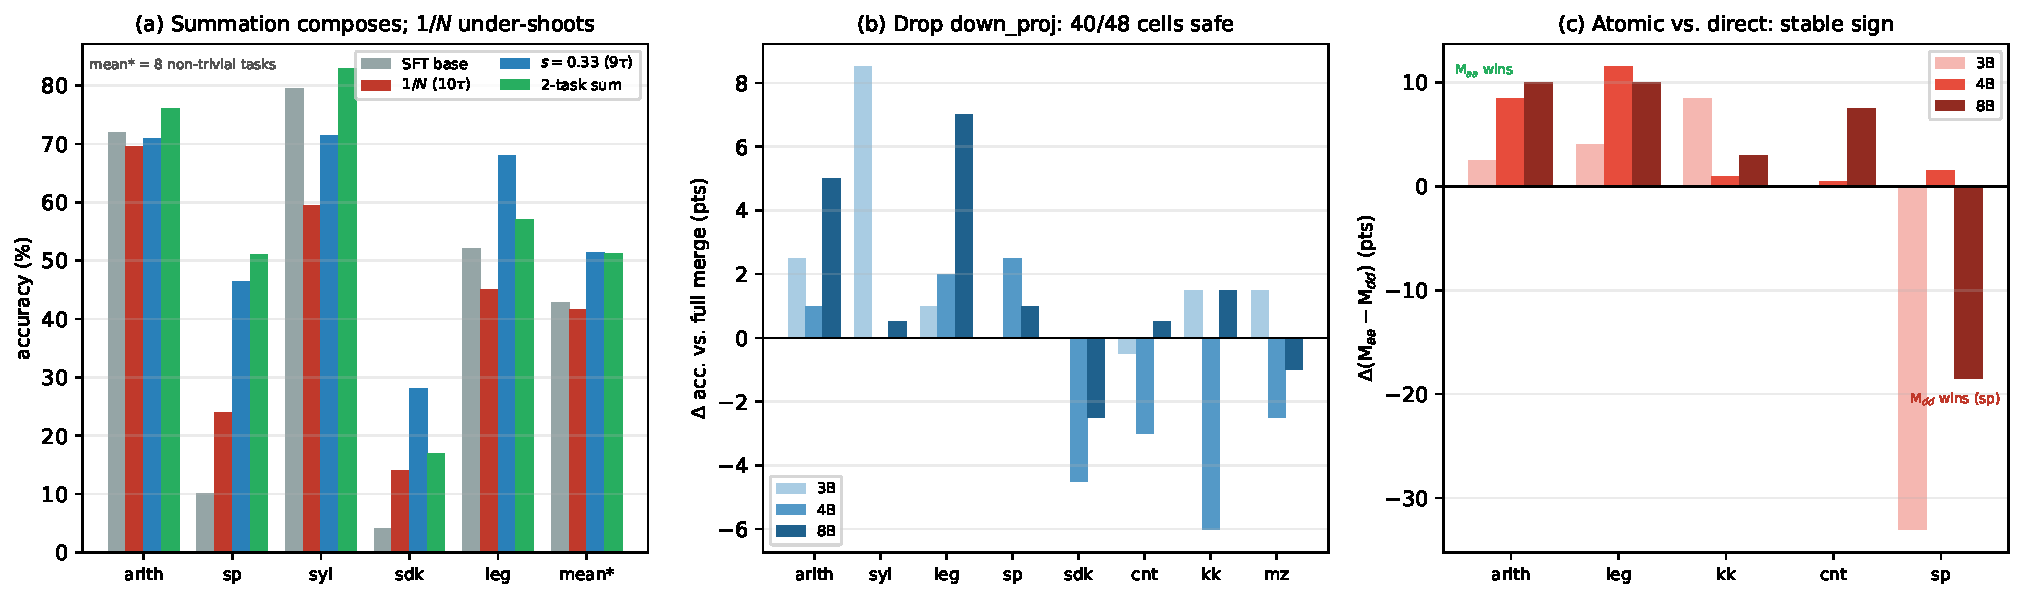
\includegraphics[width=\textwidth]{fig_p4_worked.pdf}
\caption{\textbf{The three constructive results.} (a) Summation composes: a 2-task sum
($s{=}1.0$, green) holds both skills and beats $1/N$ averaging (red) on $9/10$ tasks, while $1/N$
under-shoots every task; the binding constraint is the total displacement budget, not the source
count. (b) Dropping the \texttt{mlp.down\_proj} contribution is safe: for SP$+$Arith the change
versus the full merge is neutral-to-positive at 3B/4B/8B (bars shown; at or above $0$ is lossless),
and across the 4B pair set it is lossless on $40/48$ (pair, task) cells, the one universally safe
recipe. (c) Atomic ($\mathrm{M}_{aa}$) versus direct
($\mathrm{M}_{dd}$) vectors compose with a per-task sign that is stable across scale:
$\mathrm{M}_{aa}$ wins on arithmetic/leg-counting/knights-knaves/countdown at every scale,
$\mathrm{M}_{dd}$ wins on \texttt{shortest\_path}. Data transcribed from
Tables~\ref{tab:p4-part1} and \ref{tab:p4-f28}.}
\label{fig:p4worked}
\end{figure}

\paragraph{Simple summation composes skills (near-orthogonality).} Summing two single-task
vectors at $s{=}1.0$ yields a model that holds both skills: SP$+$Arith lifts
\texttt{shortest\_path} from $10\%$ (SFT base) to $51\%$ while keeping arithmetic at $76\%$
(Table~\ref{tab:p4-part1}, Figure~\ref{fig:p4worked}a). The mechanism is the \S\ref{sec:phase3}
finding that RLVR $\tv$'s are near-orthogonal both to $W$ and to each other: two skills written
into nearly disjoint directions add without overwriting one another. This is not special to
SP$+$Arith: we summed all 19 pairs (Table~\ref{tab:p4-damage19}), and composition is the default
across them, with median damage $19.5$ points, $15/19$ pairs below $25$, and two near-lossless
pairs (\texttt{cnt}$+$\texttt{leg} and \texttt{sp}$+$\texttt{leg}, both $0.5$). Catastrophic
clashes are the exception, confined to four \texttt{mini\_sudoku}- and \texttt{countdown}-heavy
outliers (\texttt{kk}$+$\texttt{sdk} $64.5$, \texttt{sp}$+$\texttt{sdk} $51$,
\texttt{cnt}$+$\texttt{sdk} $45.5$, \texttt{cnt}$+$\texttt{syl} $40$). Composition is thus the
\emph{default} outcome of summation, and catastrophic clashes are the exception, not the rule.

\paragraph{Scale beats $N$; $1/N$ averaging is a dead end.} The TIES/DARE-canonical recipe of
averaging all ten $\tv$'s at $s{=}1/N{=}0.1$ under-shoots: it loses to a 2-task sum ($s{=}1.0$)
on $9/10$ tasks (mean of 8 non-trivial tasks: $41.6\%$ vs.\ $51.2\%$; Table~\ref{tab:p4-part1},
Figure~\ref{fig:p4worked}a). The theory follows from the same near-orthogonality: because vectors do not destructively
interfere, the binding constraint is the \emph{total displacement budget}
($s\!\cdot\!N\approx 2$--$3$ $\tv$-equivalents), not the number of sources. Dividing by $N$ does
not avoid interference (there is little to avoid); it merely shrinks every skill below the
displacement it needs, so all skills under-shoot at once.

\begin{table}[t]
\centering\small
\caption{\textbf{Merge budget, not source count, matters} (4B, accuracy). $1/N$ averaging
under-shoots; 2-task and 9-task ($s{=}0.33$) merges tie at $\approx 3$ $\tv$-equivalents.}
\label{tab:p4-part1}
\begin{tabular}{lrrrr}
\toprule
Task & SFT & $1/N$ (10$\tv$) & $s{=}0.33$ (9$\tv$) & 2-task (SP$+$Arith)\\
\midrule
basic\_arithmetic & 72 & 69.5 & 71.0 & \textbf{76.0}\\
shortest\_path    & 10 & 24.0 & 46.5 & \textbf{51.0}\\
syllogism         & 79.5 & 59.5 & 71.5 & \textbf{83.0}\\
mini\_sudoku      & 4  & 14.0 & \textbf{28.0} & 17.0\\
leg\_counting     & 52 & 45.0 & \textbf{68.0} & 57.0\\
\midrule
\textbf{Mean (8 non-trivial)} & 42.9 & 41.6 & \textbf{51.3} & \textbf{51.2}\\
\bottomrule
\end{tabular}
\end{table}

\paragraph{Always drop \texttt{mlp.down\_proj} (the actionable recipe).} Dropping
\texttt{down\_proj} contributions from a merge is neutral-to-positive on $40$ of the $48$
(pair, task) cells we evaluated at 4B (Figure~\ref{fig:p4worked}b). Each \emph{cell} is one task's
accuracy under the \texttt{down\_proj}-dropped merge compared against the full merge for one pair,
and \emph{neutral-to-positive} means the dropped merge stays within $3$ points of, or exceeds, the
full merge, i.e.\ the drop is lossless; the $48$ cells cover the 4B merge pairs across the eight
non-trivial tasks, and the recipe is additionally mean-positive at 3B and 8B. This is the one
universally safe, geometrically motivated merge recipe we found, and it survives every scale and
every pair we tested. The theory is a direct operationalization of the \S\ref{sec:phase3}
frozen-basis invariant: the \texttt{mlp.down\_proj} basis rotates $0\dg$ under RLVR, so each task
vector's \texttt{down\_proj} component points along directions the model never repurposes while
learning the skill. That component therefore carries no skill-specific signal, only summed
numerical noise that can fight across vectors, so discarding it removes a source of conflict at no
capability cost. More aggressive masking (\texttt{up\_proj}$+$\texttt{gate\_proj} only) works for
some pairs and fails for others (the per-pair layer-selective breakdown across six further pairs is
in Appendix~\ref{app:merge}), and TIES and DARE \citep{yadav2023ties,yu2024dare} do not
consistently beat vanilla summation (within $\pm 2$ pts on three tested pairs): once
\texttt{down\_proj} is gone, the remaining attention circuit is genuinely load-bearing for some
pairs and cannot be pruned generically.

\paragraph{Atomic vs.\ direct vectors compose differently (cross-scale stable).} Merging two
atomic-curriculum vectors (M$_{aa}$) versus two direct-GRPO vectors (M$_{dd}$) for the same task
pair gives a per-task sign that is stable across scale: M$_{aa}$ wins on feature-routing tasks
(arithmetic, leg\_counting, knights\_knaves, countdown) at every scale, while M$_{dd}$ wins on
\texttt{shortest\_path} at every scale (Table~\ref{tab:p4-f28}, Figure~\ref{fig:p4worked}c). The
mean magnitude is scale-specific ($+7.9$ at 4B, $+0.3$ at 8B, $-3.3$ at 3B), but the sign pattern
is robust. Our
hypothesis for the split mirrors the \S\ref{sec:phase2} atom decomposition: the atomic curriculum
front-loads grounding (L1) and writes the skill into the same feature-routing MLP directions that
compose additively, whereas \texttt{shortest\_path}'s gain is carried by attention-circuit
restructuring that direct GRPO captures more faithfully, so its atomic vector composes worse.
Pairing this with the \S\ref{sec:phase2} regime rule yields a heterogeneous training-then-merging
recipe: train each skill in its ARS-recommended regime, then sum.

\begin{table}[t]
\centering\small
\caption{\textbf{Atomic vs.\ direct composition} $\Delta(\mathrm{M}_{aa}-\mathrm{M}_{dd})$ (pts).
Per-task sign is cross-scale stable; M$_{dd}$ wins only on \texttt{shortest\_path}.}
\label{tab:p4-f28}
\begin{tabular}{lrrrl}
\toprule
Task & 3B & 4B & 8B & Pattern\\
\midrule
basic\_arithmetic & $+2.5$ & $+8.5$ & $+10.0$ & M$_{aa}$ wins at every scale\\
leg\_counting     & $+4.0$ & $+11.5$& $+10.0$ & M$_{aa}$ wins at every scale\\
knights\_knaves   & $+8.5$ & $+1.0$ & $+3.0$  & M$_{aa}$ wins at every scale\\
countdown         & $0.0$  & $+0.5$ & $+7.5$  & M$_{aa}$ wins\\
shortest\_path     & $\mathbf{-33.0}$ & $+1.5$ & $\mathbf{-18.5}$ & \textbf{M$_{dd}$ wins}\\
\bottomrule
\end{tabular}
\end{table}

\subsection{What did not work, and where it broke}
\label{sec:p4-nulls}

\paragraph{No cheap predictor of which pairs merge cleanly (broke at larger $n$).} The natural
goal, a pre-probe that flags clashing pairs before any merge, proved unreachable. An earlier draft
of this work reported two predictors of 4B merge damage estimated on the original $n{=}7$ pairs: a
weight-space \emph{magnitude-weighted sign-agreement} at 3B ($r{=}{-}0.81$) and a behavioral
\emph{L1-grounding ARS} at 3B ($r{=}{-}0.76$). We ran 12 more pairs ($n{=}19$) specifically to
stress-test them \emph{before} submission, and that is exactly where they broke: both collapse
monotonically with sample size (Table~\ref{tab:p4-decay}, Figure~\ref{fig:p4}). Sign-agreement
decays $-0.81\!\rightarrow\!-0.45\!\rightarrow\!-0.27$ (bootstrap CI crosses zero at every
$n\geq 12$), and L1-ARS \emph{flips sign} at $n{=}12$ ($-0.76\!\rightarrow\!+0.06$). Our hypothesis
for why they ever looked strong is a favorable-small-sample artifact: with only seven pairs, a
single monotone ordering is easy to hit by chance, and the steep $n{=}7$ fit is dominated by a few
points; the population correlation is a weak directional $\approx{-}0.3$ at best, too noisy to
calibrate a go/no-go decision.

\begin{table}[t]
\centering\small
\caption{\textbf{Predictor decay.} Entries are Pearson correlations $r$ between each candidate
predictor and merge damage. A \emph{useful} predictor needs large magnitude $|r|$ (near $\pm 1$);
$r\approx 0$ means no predictive power, so for a predictor larger $|r|$ is ``better''. The sign
only encodes direction (negative $r$: a higher predictor value implies lower damage). Both
predictors that look strong at $n{=}7$ decay toward $0$ by $n{=}19$, i.e.\ lose their power; the
right column lists predictors null at every $n$.}
\label{tab:p4-decay}
\begin{tabular}{lrrr@{\hskip 2em}l}
\toprule
Predictor (Pearson $r$) & $n{=}7$ & $n{=}12$ & $n{=}19$ & Null at every $n$\\
\midrule
3B sign-agreement $\to$ damage & $-0.81$ & $-0.45$ & $-0.27$ & Phase-1 transfer ($r\approx0$)\\
3B L1-ARS $\to$ damage         & $-0.76$ & $+0.06$ & n/a    & global $\tv$ cosine\\
routing probe $\to$ group      & n/a    & $-0.31$ & n/a    & per-layer flat-cosine ($+0.23$)\\
best single residual feature   & n/a    & $<|0.5|$ & n/a   & $\tv$ magnitude / eff.\ rank\\
\bottomrule
\end{tabular}
\end{table}

\begin{figure}[t]
\centering
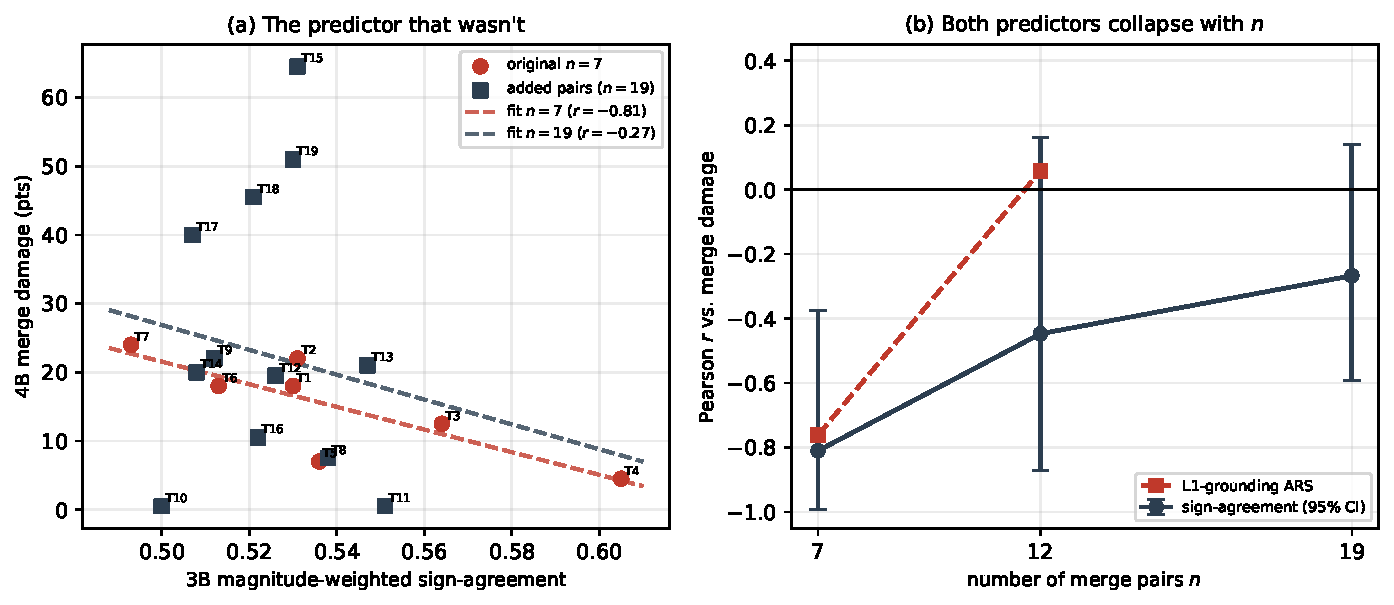
\includegraphics[width=\textwidth]{fig_p4_merge.pdf}
\caption{\textbf{No prospective predictor of merge damage survives.} (a) 3B sign-agreement vs.\
4B merge damage: the steep fit on the original $n{=}7$ pairs ($r{=}{-}0.81$) flattens to
$r{=}{-}0.27$ over all $n{=}19$; outliers like T10/T11 (damage $0.5$) and T15 (damage $64.5$)
sit at ordinary sign-agreement. (b) Both candidate predictors decay toward zero as pairs are
added: sign-agreement $-0.81\!\rightarrow\!-0.27$ (95\% CI crossing zero for every $n\geq12$)
and L1-grounding ARS flips sign ($-0.76\!\rightarrow\!+0.06$).}
\label{fig:p4}
\end{figure}

\paragraph{Task-intrinsic merge ``groups'' do not exist (broke when partners changed).} An earlier
draft classified \emph{tasks} as ``MLP-only-sufficient'' (G1) or ``needs-full-attention'' (G2) for
merging, a clean task-level taxonomy. Re-running layer-selective merges on 6 more pairs broke it:
\texttt{shortest\_path} is G2 with \texttt{arithmetic} but G1 with \texttt{knights\_knaves};
\texttt{syllogism} flips the other way; only \texttt{mini\_sudoku} is stably G2. The hypothesis
that fits this is that compatibility is \emph{interactional}: which layers a merge needs is a
property of how two specific vectors overlap at specific parameters, not a label you can attach to
either task in isolation, so it cannot be read off task features. The corroborating nulls follow
the same logic: a task-level routing probe predicts group at only $r{=}{-}0.31$, and a residual
search over ten candidate features finds no single $|r|>0.5$ and no two-feature $R^2>0.55$ at
$n{=}12$ (a ``task-incompatibility'' feature reaches $r{=}0.82$ on the full sample but $r{=}0.06$
under leave-one-out, entirely overfit on task identity). Completing the \S\ref{sec:phase3} picture,
\texttt{attn.\{k,v,o\}} are \emph{not} frozen ($k$ rotates $30\dg$--$42\dg$, $v$/$o$
$50\dg$--$70\dg$), which is why some pairs genuinely need the full attention circuit and no fixed
mask generalizes.

\paragraph{Why no global metric can see the damage (the unifying hypothesis).} The same
near-orthogonality that makes summation work is what makes damage invisible. \S\ref{sec:phase3}
established that RLVR $\tv$'s are nearly orthogonal both to $W$ and to each other, so any
\emph{averaged} statistic of two vectors looks essentially identical whether or not they will
clash. Damage, when it occurs, lives at a \emph{localized, per-parameter} level: sign conflicts at
a handful of high-magnitude positions that a global average dilutes to nothing. This predicts
exactly what we see: two tasks with perfectly normal sign-agreement can still merge
catastrophically (\texttt{knights\_knaves}$+$\texttt{mini\_sudoku}: damage $64.5$, KK drops
$47$ pts). It also predicts that a useful predictor, if one exists, would have to be a
\emph{localized per-parameter} conflict measure rather than any of the global summaries we tried.
The honest conclusion: RLVR 2-vector merging has a \emph{characterized but not prospectively
predictable} structure. We regard this as a contribution. The merging literature has implicitly
assumed task-intrinsic compatibility and cheap pre-probes, and our $n{=}19$ evidence rules out both
for reasoning RLVR vectors.

% =====================================================================
\section{Limitations}
% =====================================================================
(1) \textbf{Family confound:} 3B/7B are Qwen2.5, 4B/8B are Qwen3, so some ``scale'' effects may be
family effects; non-Qwen replication (Llama-3, Gemma-2) is future work. (2) \textbf{Sample size:}
merge analysis is $n{=}19$ pairs at one focal scale (4B); the null results are robust to this $n$
but a still-larger sweep could surface a weak predictor we missed. (3) \textbf{Seed variance:}
training-seed variance is spot-checked, not exhaustively characterized. (4) \textbf{Atom design:}
ARS is only as good as the hand-authored atoms, as \texttt{mini\_sudoku} shows. (5)
\textbf{Causality:} Phase-3 geometry is correlational; we do not run interventional experiments
(e.g.\ projecting out shared directions during multi-task training).

% =====================================================================
\section{Conclusion}
\label{sec:synthesis}
% =====================================================================
GRPO on small reasoning models is not free improvement. It degrades a third of task pairs, but
its weight-space action has a remarkably clean, scale-invariant signature, and a cheap probe
(ARS) predicts when and how to apply it. That geometry yields a robust merge recipe (drop
\texttt{mlp.down\_proj}) and a cross-scale composition effect (atomic vs.\ direct), but \emph{not}
a prospective merge-damage predictor: two predictors we initially believed at $n{=}7$ collapsed
at $n{=}19$. The result is an empirical characterization of RLVR training dynamics that is honest
about what it can and cannot predict, and we hope a useful map for practitioners and a caution to
the model-merging literature.

\paragraph{Five universal empirical laws.} Across all phases and scales: (1) GRPO is
spectrum-preserving; (2) $\tv$ is near-orthogonal to $W$'s top subspace; (3) the
\texttt{mlp.down\_proj} basis is always frozen; (4) \texttt{down\_proj} $\tv$ contributions are
always droppable from a merge; (5) single-task GRPO produces a $\tv$ of Frobenius magnitude
$\sim$0.7--1.2 at 4B, insensitive to task identity, with only the direction and depth varying.

\paragraph{The connective thread.} ARS diagnoses \emph{what RLVR needs} (\S\ref{sec:phase2}); the
weight geometry shows \emph{what GRPO structurally does} (\S\ref{sec:phase3}); and that geometry
makes merging tractable (drop \texttt{down\_proj}) but only \emph{partly} predictable
(\S\ref{sec:phase4}). The bridge we once hoped for, a grounding bottleneck unifying single-task
success with merge compatibility, did not survive (\S\ref{sec:p4-nulls}): ARS is a valid
\emph{single-task training-regime} predictor, but not a \emph{merge-compatibility} predictor. We
think honesty about this boundary is more useful to the field than an over-claimed unification.

\paragraph{Practical recipe.} (i) Run the ARS probe ($\sim$1 hr); pick the regime by band, watching
for reasoning compression on long-chain tasks. (ii) Train single-task $\tv$'s, using atomic
curricula for feature-routing tasks and direct GRPO for spatial-search tasks. (iii) Merge with the
\texttt{all\_but\_down} mask at $s{\approx}1.0$ for two vectors (scale down for more); \emph{measure}
each merge. No cheap probe substitutes.

\paragraph{Reproducibility.} All SFT/GRPO checkpoints, ARS probes, merge checkpoints, evaluation
outputs, and analysis scripts are released. Appendices give full per-scale transfer matrices
(\ref{app:p1}), per-task atom breakdowns (\ref{app:ars}), the shortest-path deep dive
(\ref{app:sp}), the MMLU forgetting study (\ref{app:mmlu}), the full 19-pair merge table
(\ref{app:merge}), and hyperparameters (\ref{app:hparams}).

\bibliographystyle{tmlr}
\bibliography{references}

\appendix
% =====================================================================
\section{7B/8B Transfer Matrices and the Learning-Rate Sweep}
\label{app:p1}
% =====================================================================
The four matrices below complete the cross-scale picture (\texttt{caesar\_cipher} and
\texttt{cryptarithm} omitted as before). At the aggressive $\mathrm{lr}{=}5\times10^{-6}$ (v1) the
7B/8B models are the most volatile in the study, both the largest gains and the largest harms;
the gentle $\mathrm{lr}{=}1\times10^{-6}$/16-generation setting (v2) flattens the matrix to within
$\pm 8$ pts everywhere, eliminating catastrophic harm but also nearly all learning.

\begin{table}[h]
\centering\small
\caption{\textbf{Qwen2.5-7B v1} ($\mathrm{lr}{=}5{\times}10^{-6}$, 8 generations).}
\begin{tabular}{lrrrrrrrr}
\toprule
Trained on & cnt & mz & sdk & pth & ari & syl & kk & leg\\
\midrule
countdown      & $+60^\star$ & $-4$ & $-6$ & $0$ & $-2$ & $+6$ & $+8$ & $-8$\\
maze           & $-4$ & $+10^\star$ & $-6$ & $-4$ & $-2$ & $+4$ & $0$ & $-10$\\
mini\_sudoku   & $+2$ & $-4$ & $+16^\star$ & $-4$ & $-6$ & $-8$ & $+4$ & $-6$\\
shortest\_path & $-4$ & $-2$ & $-4$ & $+36^\star$ & $-8$ & $-24$ & $0$ & $-2$\\
basic\_arith   & $-2$ & $+2$ & $-12$ & $-4$ & $-30^\star$ & $-2$ & $0$ & $-30$\\
syllogism      & $0$ & $+6$ & $-12$ & $-4$ & $-46$ & $+26^\star$ & $-28$ & $-32$\\
knights\_knaves& $-2$ & $-2$ & $-10$ & $-4$ & $-32$ & $-8$ & $+28^\star$ & $-32$\\
leg\_counting  & $-4$ & $+2$ & $-4$ & $-4$ & $-10$ & $-2$ & $+2$ & $+8^\star$\\
\midrule
\textbf{Baseline} & 4\% & 14\% & 12\% & 4\% & 60\% & 64\% & 32\% & 32\%\\
\bottomrule
\end{tabular}
\end{table}

\begin{table}[h]
\centering\small
\caption{\textbf{Qwen3-8B v1} ($\mathrm{lr}{=}5{\times}10^{-6}$, 8 generations). \texttt{mini\_sudoku}
reaches $+60$ (0\%$\rightarrow$60\%); \texttt{maze} is a corrupted zero-reward run.}
\begin{tabular}{lrrrrrrrr}
\toprule
Trained on & cnt & mz & sdk & pth & ari & syl & kk & leg\\
\midrule
countdown      & $+50^\star$ & $-10$ & $+22$ & $+8$ & $-4$ & $-2$ & $+2$ & $-4$\\
maze           & $-24$ & $-10^\star$ & $0$ & $-8$ & $-8$ & $-22$ & $-30$ & $-40$\\
mini\_sudoku   & $+18$ & $+10$ & $+60^\star$ & $+16$ & $+10$ & $+6$ & $+6$ & $-4$\\
shortest\_path & $-4$ & $+10$ & $+8$ & $+36^\star$ & $+2$ & $-8$ & $+6$ & $0$\\
basic\_arith   & $-14$ & $+4$ & $+14$ & $+4$ & $-2^\star$ & $-4$ & $-4$ & $-8$\\
syllogism      & $-16$ & $-6$ & $+6$ & $-2$ & $-2$ & $+18^\star$ & $-6$ & $-16$\\
knights\_knaves& $-18$ & $-8$ & $+16$ & $+4$ & $-2$ & $0$ & $-6^\star$ & $-10$\\
leg\_counting  & $+6$ & $-2$ & $0$ & $+10$ & $+4$ & $-10$ & $0$ & $0^\star$\\
\midrule
\textbf{Baseline} & 32\% & 10\% & 0\% & 8\% & 64\% & 78\% & 64\% & 48\%\\
\bottomrule
\end{tabular}
\end{table}

\begin{table}[h]
\centering\small
\caption{\textbf{Qwen2.5-7B v2} ($\mathrm{lr}{=}1{\times}10^{-6}$, 16 generations).}
\begin{tabular}{lrrrrrrrr}
\toprule
Trained on & cnt & mz & sdk & pth & ari & syl & kk & leg\\
\midrule
countdown      & $-2^\star$ & $+4$ & $+4$ & $0$ & $0$ & $+2$ & $+4$ & $-6$\\
maze           & $-4$ & $+6^\star$ & $+6$ & $+4$ & $0$ & $+2$ & $+2$ & $-6$\\
mini\_sudoku   & $-4$ & $0$ & $+8^\star$ & $+4$ & $0$ & $-2$ & $+2$ & $-2$\\
shortest\_path & $-2$ & $+2$ & $+8$ & $+8^\star$ & $-2$ & $0$ & $+2$ & $-6$\\
basic\_arith   & $-2$ & $+2$ & $+2$ & $+4$ & $-4^\star$ & $+2$ & $0$ & $-2$\\
syllogism      & $-4$ & $+2$ & $+4$ & $0$ & $-2$ & $+8^\star$ & $+2$ & $-4$\\
knights\_knaves& $-2$ & $0$ & $+6$ & $+2$ & $0$ & $-4$ & $+4^\star$ & $0$\\
leg\_counting  & $-4$ & $+2$ & $+4$ & $+4$ & $0$ & $0$ & $-4$ & $+2^\star$\\
\midrule
\textbf{Baseline} & 4\% & 12\% & 4\% & 2\% & 60\% & 64\% & 30\% & 36\%\\
\bottomrule
\end{tabular}
\end{table}

\begin{table}[h]
\centering\small
\caption{\textbf{Qwen3-8B v2} ($\mathrm{lr}{=}1{\times}10^{-6}$, 16 generations). Note the
systematically negative \texttt{kk} column: GRPO on anything degrades this fragile 74\% task.}
\begin{tabular}{lrrrrrrrr}
\toprule
Trained on & cnt & mz & sdk & pth & ari & syl & kk & leg\\
\midrule
countdown      & $+4^\star$ & $-2$ & $+6$ & $-8$ & $+2$ & $0$ & $-12$ & $-2$\\
maze           & $0$ & $0^\star$ & $+4$ & $-6$ & $+2$ & $0$ & $-10$ & $-2$\\
mini\_sudoku   & $+4$ & $+2$ & $+2^\star$ & $-2$ & $+4$ & $+4$ & $-6$ & $0$\\
shortest\_path & $-4$ & $-4$ & $0$ & $-4^\star$ & $+2$ & $+4$ & $-8$ & $-2$\\
basic\_arith   & $+2$ & $+2$ & $0$ & $-6$ & $+4^\star$ & $+2$ & $-8$ & $-2$\\
syllogism      & $+6$ & $-2$ & $0$ & $-2$ & $+4$ & $+2^\star$ & $-10$ & $0$\\
knights\_knaves& $+6$ & $-4$ & $+4$ & $-6$ & $+4$ & $0$ & $-14^\star$ & $-2$\\
leg\_counting  & $+2$ & $-4$ & $0$ & $-6$ & $+4$ & $+2$ & $-18$ & $0^\star$\\
\midrule
\textbf{Baseline} & 22\% & 10\% & 0\% & 12\% & 62\% & 74\% & 74\% & 52\%\\
\bottomrule
\end{tabular}
\end{table}

The aggregate learning-rate effect is summarized below.

\begin{table}[h]
\centering\small
\caption{\textbf{The learning-rate effect} (v1 $=5{e}{-}6$, v2 $=1{e}{-}6$/16 gen).}
\begin{tabular}{lrrrr}
\toprule
Metric & 7B v1 & 7B v2 & 8B v1 & 8B v2\\
\midrule
Max diagonal gain      & $+60$ & $+8$  & $+60$ & $+4$\\
Worst diagonal harm    & $-30$ & $-4$  & $-10$ & $-4$\\
Mean $|\Delta|$        & 8.9\% & 3.0\% & 11.2\%& 3.8\%\\
Cells with $>10\%$ harm& 14    & 0     & 11    & 2\\
\bottomrule
\end{tabular}
\end{table}

% =====================================================================
\section{Per-Task Atom Breakdowns and the ARS Recipe}
\label{app:ars}
% =====================================================================
\paragraph{The ARS measurement recipe.} ARS is a pure inference probe (no gradients, no training
data). For each task: (1) hand-author 6--14 atom templates split between L1 (grounding) and L2
(local reasoning), each a deterministic function of a \texttt{reasoning-gym} sample with a
programmatically verifiable answer; (2) draw 50 valid (question, ground-truth) pairs per atom
(seed 9999, oversampling for atoms that reject ill-fitting samples); (3) zero-shot generate from
the SFT base with a fixed ``answer concisely inside \texttt{<answer>} tags'' prompt, greedy
decoding, 128 max new tokens, and extract the \emph{last} \texttt{<answer>} match (first-match was
fooled by echoed template tags); (4) score each atom with a \emph{lenient}, type-aware verifier
(numeric/list/character/token canonicalization, not strict string equality); (5) average into
$\mathrm{L1\_avg}$, $\mathrm{L2\_avg}$, and $\mathrm{ARS}=\mathrm{mean}(\mathrm{L1}\cup\mathrm{L2})$.
Cost: $\approx 8$--$10$ min/task on one GPU; the 7-task probe runs in $\approx 1$ hour.

\begin{table}[h]
\centering\small
\caption{\textbf{Per-task ARS summary} (Qwen3-4B SFT base, 50 samples/atom). L1 = grounding floor,
L2 = local-reasoning floor.}
\begin{tabular}{lcccccl}
\toprule
Task & \#L1 & \#L2 & L1\_avg & L2\_avg & ARS & Reading\\
\midrule
syllogism        & 4 & 3 & 96\%   & 52\%   & 74\%   & aces grounding; single-hop validity is the gap\\
knights\_knaves  & 4 & 4 & 57\%   & 68\%   & 62.5\% & unusual L2$>$L1; cannot attribute statements\\
basic\_arithmetic& 4 & 4 & 67.5\% & 65\%   & 66\%   & both floors clear; fails via reasoning compression\\
countdown        & 3 & 3 & 34\%   & 78\%   & 56\%   & weak L1, strong L2; bottleneck is L3 search\\
maze             & 4 & 3 & 14\%   & 27\%   & 20.7\% & cannot locate start/goal\\
shortest\_path   & 4 & 3 & 0\%    & 27\%   & 14\%   & cannot read the grid at all\\
mini\_sudoku     & 4 & 4 & 24\%   & 15.5\% & 19.8\% & atoms miss the constraint-propagation bottleneck\\
\bottomrule
\end{tabular}
\end{table}

\begin{table}[h]
\centering\small
\caption{Atom-level base accuracy, high/medium-ARS tasks.}
\begin{tabular}{lllr}
\toprule
Task & Atom & Layer & Base\\
\midrule
\multirow{7}{*}{syllogism}
 & premise1\_subject     & L1 & 100\%\\
 & premise2\_subject     & L1 & 100\%\\
 & quantifier\_type      & L1 & 86\%\\
 & conclusion\_predicate & L1 & 98\%\\
 & single\_hop\_inference& L2 & 46\%\\
 & negation              & L2 & 42\%\\
 & validity\_check       & L2 & 68\%\\
\midrule
\multirow{8}{*}{knights\_knaves}
 & count\_inhabitants    & L1 & 66\%\\
 & list\_names           & L1 & 90\%\\
 & speaker\_identification& L1 & 0\%\\
 & terminology           & L1 & 72\%\\
 & statement\_about      & L2 & 72\%\\
 & if\_sage\_then        & L2 & 96\%\\
 & if\_fool\_then        & L2 & 100\%\\
 & consistency\_check    & L2 & 4\%\\
\midrule
\multirow{8}{*}{basic\_arithmetic}
 & number\_extraction    & L1 & 62\%\\
 & operator\_identification& L1 & 70\%\\
 & term\_count           & L1 & 40\%\\
 & has\_parentheses      & L1 & 98\%\\
 & single\_op\_eval      & L2 & 76\%\\
 & order\_of\_operations & L2 & 2\%\\
 & innermost\_eval       & L2 & 82\%\\
 & sign\_handling        & L2 & 100\%\\
\midrule
\multirow{6}{*}{countdown}
 & number\_inventory     & L1 & 10\%\\
 & target\_reading       & L1 & 90\%\\
 & how\_many\_numbers    & L1 & 2\%\\
 & single\_op            & L2 & 94\%\\
 & two\_number\_reachability & L2 & 50\%\\
 & distance\_to\_target  & L2 & 90\%\\
\bottomrule
\end{tabular}
\end{table}

\begin{table}[h]
\centering\small
\caption{Atom-level base accuracy, low-ARS tasks. Note the floor-zero grounding for the grid tasks.}
\begin{tabular}{lllr}
\toprule
Task & Atom & Layer & Base\\
\midrule
\multirow{7}{*}{maze}
 & locate\_start         & L1 & 0\%\\
 & locate\_goal          & L1 & 0\%\\
 & read\_cell            & L1 & 54\%\\
 & grid\_size            & L1 & 2\%\\
 & valid\_moves          & L2 & 8\%\\
 & is\_move\_valid       & L2 & 62\%\\
 & shortest\_path\_length& L2 & 12\%\\
\midrule
\multirow{7}{*}{shortest\_path}
 & locate\_start         & L1 & 0\%\\
 & locate\_goal          & L1 & 0\%\\
 & read\_cell            & L1 & 0\%\\
 & grid\_dimensions      & L1 & 0\%\\
 & valid\_neighbors      & L2 & 0\%\\
 & is\_move\_legal       & L2 & 54\%\\
 & direction\_to\_goal   & L2 & 28\%\\
\midrule
\multirow{8}{*}{mini\_sudoku}
 & read\_cell            & L1 & 24\%\\
 & count\_empty          & L1 & 0\%\\
 & row\_values           & L1 & 30\%\\
 & col\_values           & L1 & 42\%\\
 & missing\_in\_row      & L2 & 16\%\\
 & missing\_in\_col      & L2 & 22\%\\
 & can\_place            & L2 & 20\%\\
 & only\_option          & L2 & 4\%\\
\bottomrule
\end{tabular}
\end{table}

\clearpage

% =====================================================================
\section{Per-Task Atomic Curriculum Experiments}
\label{app:atomic}
% =====================================================================
Section~\ref{sec:phase2} reports the headline result from one summary table. Here we give the
full four-condition experiment behind every task, paired with the per-atom bottleneck (the atom
tables in Appendix~\ref{app:ars}) that explains it. All conditions share the GRPO recipe of
Appendix~\ref{app:hparams} ($\mathrm{lr}{=}5\!\times\!10^{-6}$ constant, DAPO loss, $\beta{=}0$,
KL${=}0$, 8 generations/prompt, temperature 1.0) and matched compute:

\begin{itemize}\itemsep2pt
\item \textbf{Base} --- the SFT checkpoint, no GRPO.
\item \textbf{Direct-RLVR} --- 300 GRPO steps on the full task.
\item \textbf{Atomic-Only} --- 100 steps on L1 atoms $\rightarrow$ 100 steps on L2 atoms, then
\emph{zero-shot} evaluation on the full task (no full-task training at all).
\item \textbf{Atomic-Warm} --- L1 (100) $\rightarrow$ L2 (100) $\rightarrow$ full task (100),
300 steps total.
\end{itemize}

\begin{table}[h]
\centering\small
\caption{\textbf{Full atomic-curriculum results, all 7 tasks.} Full-task eval accuracy.
Bold $=$ best regime per task. $\Delta$ is best minus Direct-RLVR, i.e.\ how much the atomic
curriculum buys over training the full task directly.}
\label{tab:atomic-full}
\begin{tabular}{lrrrrrrrlr}
\toprule
Task & ARS & L1 & L2 & Base & Direct & At.-Only & At.-Warm & Best & $\Delta$\\
\midrule
syllogism        & 74\%   & 96\%   & 52\%   & 79.5 & 96.5 & 81.0 & \textbf{97.0} & At.-Warm & $+0.5$\\
knights\_knaves  & 62.5\% & 57\%   & 68\%   & 78.0 & \textbf{97.5} & 79.0 & 95.0 & Direct & ---\\
basic\_arithmetic& 66\%   & 67.5\% & 65\%   & 72.0 & 32.0 & \textbf{78.0} & 70.0 & At.-Only & $\mathbf{+46}$\\
countdown        & 56\%   & 34\%   & 78\%   & 26.0 & \textbf{$\sim$70} & 24.0 & 26.0 & Direct & ---\\
maze             & 20.7\% & 14\%   & 27\%   & 21.5 & 1.0  & \textbf{41.0} & 38.5 & At.-Only & $\mathbf{+40}$\\
shortest\_path   & 14\%   & 0\%    & 27\%   & 10.0 & 44.0 & 12.0 & \textbf{46.0} & At.-Warm & $+2$\\
mini\_sudoku     & 19.8\% & 24\%   & 15.5\% & 4.0  & \textbf{25.5} & 17.0 & 24.0 & Direct & ---\\
\bottomrule
\end{tabular}
\end{table}

\paragraph{High-ARS tasks ($>60\%$).}
\emph{syllogism} (ARS 74\%) aces grounding (L1 96\%) but is mediocre at single-hop validity
(L2 52\%); both Direct-RLVR and Atomic-Warm reach $\approx 97\%$, so GRPO supplies the missing
L2/L3 inference and atoms add only $+0.5$. \emph{knights\_knaves} (ARS 62.5\%) shows the unusual
L2$>$L1 pattern: the model knows the if-sage/if-fool rules (96\%/100\%) but cannot attribute
statements to speakers (\texttt{speaker\_identification} 0\%, \texttt{consistency\_check} 4\%);
despite these gaps the 78\% base plus Direct-RLVR ($+19.5$) learns the attribution implicitly,
and Atomic-Only barely moves it. \emph{basic\_arithmetic} (ARS 66\%) is the instructive
exception in this band: both floors clear, yet Direct-RLVR \emph{destroys} it ($72\to32$). The
bottleneck is not grounding but \texttt{order\_of\_operations} (2\%), and full-task GRPO triggers
reasoning compression (\S\ref{sec:phase2}); Atomic-Only is the only regime that fixes the gap
without compressing, reaching 78\% ($+46$ over Direct).

\paragraph{Medium-ARS task ($40$--$60\%$).}
\emph{countdown} (ARS 56\%) has weak L1 (cannot inventory or count the numbers,
\texttt{number\_inventory} 10\%, \texttt{how\_many\_numbers} 2\%) but strong L2 arithmetic
(\texttt{single\_op} 94\%). The true bottleneck is L3: the multi-step search for a combination
reaching the target, which atoms do not teach. Only Direct-RLVR moves the needle ($26\to\sim70$);
both atomic regimes stay at base. This is the band where the decision rule says ``skip the
atoms.''

\paragraph{Low-ARS tasks ($<25\%$).}
\emph{maze} (ARS 20.7\%) is the headline rescue: grounding is at the floor
(\texttt{locate\_start}/\texttt{locate\_goal} 0\%), so Direct-RLVR collapses to $1\%$ ---
\emph{below} the $21.5\%$ base, because GRPO with no grounding has no correct trajectory to
reinforce and thrashes. Atomic-Only teaches the grounding directly and reaches $41\%$ ($+40$),
with no full-task training at all. \emph{shortest\_path} (ARS 14\%, the lowest) has complete L1
failure (every grounding atom at 0\%); short Atomic-Only atoms fail ($12\%$) because they teach
grounding but compress reasoning, whereas Atomic-Warm ($46\%$) and the multi-step variants of
Appendix~\ref{app:sp} ($55.5\%$) succeed. \emph{mini\_sudoku} (ARS 19.8\%) is the one task that
breaks the rule: despite low ARS, Direct-RLVR ($25.5\%$) beats both atomic regimes. The cause is
diagnostic rather than a counterexample to the mechanism: sudoku's real bottleneck is multi-cell
constraint propagation, a holistic L2--L3 operation, and our single-hop cell-reading atoms simply
do not probe it, so the ARS we measure is uncorrelated with the actual difficulty. The lesson is
the method's honest boundary: \emph{ARS is only as predictive as the atoms are well chosen}.

\clearpage

% =====================================================================
\section{The Shortest-Path Deep Dive (15+ Conditions)}
\label{app:sp}
% =====================================================================
We took \texttt{shortest\_path} (the lowest-ARS task, $14\%$) from $10\%$ base to $55.5\%$ through
16 training conditions (Table~\ref{tab:sp}). Four reusable principles emerged.

\begin{table}[h]
\centering\small
\caption{\textbf{Shortest\_path: all 16 conditions} (Qwen3-4B). RFT-Base is best.}
\label{tab:sp}
\begin{tabular}{lrl}
\toprule
Condition & Acc. & Note\\
\midrule
Base (SFT)                                  & 10\%   & reference\\
Direct-RLVR                                 & 44\%   & Phase-1 baseline (300 steps)\\
Atomic-Warm-300 (short L2 atoms)            & 46\%   & short atoms $+$ full GRPO\\
A: progressive full-task ($3{\times}3{\to}4{\times}4{\to}$full) & 46.5\% & no atoms\\
B: L2-long atoms $\to$ full                 & 51.5\% & path-tracing atoms, hard transition\\
B2: B with $300{+}300$ steps                & 47\%   & more steps hurt\\
C: partial-credit reward                    & 35.5\% & reward too easy for GRPO\\
D: progressive $+$ partial credit           & 24\%   & worst; PC kills gradient signal\\
E: L2-long atoms $\to$ progressive full     & 27.5\% & progressive after atoms hurts\\
F: feasibility atoms $\to$ full             & 42\%   & fewer false-infeasible, more wrong paths\\
G: heavy GRPO$+$SFT interleave              & 5.5\%  & SFT collapsed the model\\
G2: light GRPO$+$SFT interleave             & 40\%   & improving (500 samples, lr $1{e}{-}6$)\\
G3: G2 $+$ 150 GRPO                          & 45\%   & matches Direct-RLVR\\
L: feasible-only training                   & 40.5\% & lost infeasibility detection\\
RFT on B's checkpoint                        & 51.5\% & on-policy SFT adds nothing to a trained model\\
\textbf{RFT-Base}                            & \textbf{55.5\%} & B's traces $\to$ base SFT $\to$ GRPO 300\\
\bottomrule
\end{tabular}
\end{table}

\textbf{(i) Long-answer atoms beat short.} Short yes/no atoms induce reasoning compression
(Atomic-Only $12\%$, below base); multi-step path-tracing atoms reach $51.5\%$ (condition B).
\textbf{(ii) One hard difficulty transition} (atoms $\to$ full grids) beats any progressive easing
(E $27.5\%$, which over-fits easy instances). \textbf{(iii) Partial-credit rewards hurt GRPO}
(C $35.5\%$, D $24\%$) by removing the advantage variance the group-relative estimator needs.
\textbf{(iv) RFT-Base} ( generate verified-correct traces from a trained model, SFT the
\emph{base} on them, then GRPO) is best at $55.5\%$ because it spends the full step budget on the
real task from a clean initialization.

\paragraph{Error analysis of condition B (51.5\%).} On 100 eval problems the failures were 23
false-infeasible (claims no path when one exists), 25 wrong-path, and 6 missed-infeasible;
feasible-problem accuracy was only $25\%$ vs.\ $83\%$ on infeasible ones. Eliminating the
false-infeasible ``give-up reflex'' alone would lift accuracy to $68.3\%$, motivating the
feasibility-atom and feasible-only experiments (F, L), which reduced false-infeasibles but traded
them for wrong paths.

\clearpage

% =====================================================================
\section{MMLU: No Catastrophic Forgetting}
\label{app:mmlu}
% =====================================================================
To check whether reasoning RLVR erodes general knowledge, we evaluated 48 checkpoints, spanning
3 sizes, all 4 phases (SFT $\to$ single-task GRPO $\to$ atomic curriculum $\to$ task-vector
merging), and 10 tasks, on three math MMLU subsets \citep{hendrycks2021mmlu}:
\texttt{abstract\_algebra} (100 q), \texttt{elementary\_mathematics} (378 q), and
\texttt{high\_school\_mathematics} (270 q). \textbf{No condition produces catastrophic forgetting:}
every checkpoint stays within $\pm 3\%$ of its SFT baseline (Tables~\ref{tab:mmlu-base}--\ref{tab:mmlu-p1}).

\begin{table}[h]
\centering\small
\caption{SFT baselines and per-size GRPO ranges on math MMLU (\texttt{abstract\_algebra} /
\texttt{elementary} / \texttt{high\_school}).}
\label{tab:mmlu-base}
\begin{tabular}{lccl}
\toprule
Size & SFT baseline & GRPO range (all tasks) & Verdict\\
\midrule
3B & 47.0 / 60.8 / 50.4 & 44--47 / 59--61 / 50--51 & slight ($1$--$3\%$) on abstract algebra\\
4B & 56.0 / 70.6 / 51.5 & 56--58 / 70--71 / 51--53 & maintained or improved\\
8B & 52.0 / 70.4 / 51.9 & 53--55 / 70--71 / 50--52 & maintained\\
\bottomrule
\end{tabular}
\end{table}

\begin{table}[h]
\centering\small
\caption{Phase-1 single-task GRPO (4B) on math MMLU, all 10 tasks maintain the SFT-4B baseline
(56.0 / 70.6 / 51.5).}
\label{tab:mmlu-p1}
\begin{tabular}{lccc}
\toprule
GRPO task (4B) & abstract\_algebra & elementary & high\_school\\
\midrule
basic\_arithmetic & 57.0 & 70.9 & 52.2\\
countdown        & 56.0 & 70.9 & 52.2\\
shortest\_path    & 58.0 & 69.8 & 51.9\\
syllogism        & 58.0 & 70.4 & 51.1\\
maze             & 57.0 & 69.8 & 51.9\\
knights\_knaves   & 57.0 & 70.4 & 52.2\\
mini\_sudoku      & 56.0 & 70.6 & 52.2\\
leg\_counting     & 58.0 & 70.6 & 52.6\\
caesar\_cipher    & 56.0 & 70.4 & 51.5\\
cryptarithm      & 56.0 & 70.6 & 51.5\\
\bottomrule
\end{tabular}
\end{table}

The atomic-curriculum (Phase 2) and layer-selective-merge (Phase 4) checkpoints behave identically
(all within $\pm 3\%$; omitted for space). GRPO-based reasoning training on these tasks is thus
safe with respect to general math knowledge.

\clearpage

% =====================================================================
\section{Full Merge Sweep and Layer-Selectivity Tables}
\label{app:merge}
% =====================================================================
The per-pair damage and sign-agreement for all 19 pairs is given in the main text
(Table~\ref{tab:p4-damage19}). Here we give the full Part-1 budget sweep and the per-pair
layer-selectivity breakdown that underlies the pair-dependence finding (\S\ref{sec:p4-nulls}).

\begin{table}[h]
\centering\small
\caption{\textbf{Full Part-1 merge sweep} (4B, 10-task accuracy): $1/N$ averaging vs.\ the
$s{=}0.33$ 9-vector merge vs.\ the 2-vector SP$+$Arith sum.}
\begin{tabular}{lrrrr}
\toprule
Task & SFT & $1/N$ (10$\tv$, $s{=}0.1$) & $s{=}0.33$ (9$\tv$) & 2-task (SP$+$Arith)\\
\midrule
basic\_arithmetic & 72   & 69.5 & 71.0 & \textbf{76.0}\\
countdown        & 26   & 39.0 & 39.0 & \textbf{39.5}\\
shortest\_path    & 10   & 24.0 & 46.5 & \textbf{51.0}\\
maze             & 21.5 & 7.5  & 4.0  & \textbf{8.5}\\
mini\_sudoku      & 4    & 14.0 & \textbf{28.0} & 17.0\\
syllogism        & 79.5 & 59.5 & 71.5 & \textbf{83.0}\\
knights\_knaves   & 78   & 74.0 & \textbf{82.0} & 77.5\\
leg\_counting     & 52   & 45.0 & \textbf{68.0} & 57.0\\
caesar\_cipher    & 0    & 0.0  & 0.0  & 0.5\\
cryptarithm      & 0    & 0.0  & 0.0  & 0.0\\
\midrule
\textbf{Mean (8 non-trivial)} & 42.9 & 41.6 & \textbf{51.3} & \textbf{51.2}\\
\bottomrule
\end{tabular}
\end{table}

\begin{table}[h]
\centering\small
\caption{\textbf{Layer-selectivity is pair-dependent} (F34). Per-(pair, task) $\Delta$ vs.\ the
full merge for the \texttt{up}, \texttt{up+q}, and \texttt{all\_but\_down} masks, and the
resulting Group label. \texttt{shortest\_path} and \texttt{syllogism} flip group with their
partner; only \texttt{mini\_sudoku} is stably G2.}
\begin{tabular}{llrrrc}
\toprule
Pair & Task & $\Delta$up & $\Delta$up$+$q & $\Delta$abd & Group\\
\midrule
T1 sdk$+$leg & mini\_sudoku    & $-8.0$  & $-9.0$  & $+3.5$  & G2\\
T1 sdk$+$leg & leg\_counting   & $0.0$   & $+1.0$  & $-8.0$  & G1\\
T2 sdk$+$kk  & mini\_sudoku    & $-24.0$ & $-27.0$ & $-16.5$ & G2\\
T2 sdk$+$kk  & knights\_knaves & $+9.0$  & $+7.0$  & $-11.5$ & G1\\
T3 ari$+$leg & basic\_arithmetic & $+23.0$ & $+23.0$ & $+11.5$ & G1\\
T3 ari$+$leg & leg\_counting   & $+2.0$  & $-4.5$  & $+6.5$  & G1\\
T4 ari$+$syl & basic\_arithmetic & $+16.5$ & $+16.0$ & $+15.0$ & G1\\
T4 ari$+$syl & syllogism       & $-6.0$  & $-5.5$  & $+0.5$  & G2\\
T6 sp$+$kk   & shortest\_path  & $+23.0$ & $+22.5$ & $+31.0$ & \textbf{G1}\\
T6 sp$+$kk   & knights\_knaves & $0.0$   & $-1.0$  & $+1.0$  & G1\\
T7 cnt$+$ari & countdown       & $+27.0$ & $+27.0$ & $+32.0$ & G1\\
T7 cnt$+$ari & basic\_arithmetic & $+10.5$ & $+11.0$ & $+10.0$ & G1\\
\bottomrule
\end{tabular}
\end{table}

\paragraph{Per-task mean damage is descriptive, not predictive.} Averaging each task's merge
damage over the pairs it appears in (Table~\ref{tab:p4-taskdamage}) shows that some tasks are, on
average, riskier merge partners: \texttt{knights\_knaves} ($20.7$) and \texttt{mini\_sudoku}
($19.8$) sit far above \texttt{leg\_counting} ($7.8$) and \texttt{shortest\_path} ($8.5$). This is
\emph{not} a usable predictor: the per-task ranges are wide and overlapping (e.g.\
\texttt{knights\_knaves} spans $18$--$64.5$, the $64.5$ being the \texttt{kk}$+$\texttt{mini\_sudoku}
catastrophe), and the pair-dependence result above (F34) shows a task's contribution flips with its
partner. The table is a summary of where damage tended to land, consistent with the headline that
merge compatibility is a property of the \emph{pair}, not the task.

\begin{table}[h]
\centering\small
\caption{\textbf{Per-task mean merge damage} (4B, over the $n{=}12$ pairs in the residual study).
Reported for description only; the wide min--max ranges and the pair-dependent layer split
(previous table) make this non-predictive for any individual pair.}
\label{tab:p4-taskdamage}
\begin{tabular}{lrrrr}
\toprule
Task & \# pairs & Mean & Min & Max\\
\midrule
leg\_counting    & 5 & 7.8  & 0.5  & 18.0\\
shortest\_path   & 3 & 8.5  & 0.5  & 18.0\\
syllogism        & 4 & 9.6  & 4.5  & 19.5\\
countdown        & 2 & 12.2 & 0.5  & 24.0\\
basic\_arithmetic& 4 & 15.8 & 4.5  & 24.0\\
mini\_sudoku     & 3 & 19.8 & 18.0 & 22.0\\
knights\_knaves  & 3 & 20.7 & 18.0 & 22.0\\
\bottomrule
\end{tabular}
\end{table}

\clearpage

% =====================================================================
\section{Hyperparameters}
\label{app:hparams}
% =====================================================================
\begin{table}[h]
\centering\small
\caption{GRPO, SFT, and evaluation hyperparameters (shared across phases unless noted).}
\begin{tabular}{lll}
\toprule
\multicolumn{2}{l}{\textbf{GRPO (DAPO)}} & \\
learning rate & $5\times10^{-6}$ constant & ($1\times10^{-6}$ in 7B/8B v2)\\
max steps & 300 single-task & 100 per atomic stage\\
num generations & 8 & 16 in v2\\
per-device batch / grad-accum & 1 / 1 & \\
$\beta$ / KL coeff & 0 / 0 & pure GRPO, no reference model\\
$\epsilon_{\mathrm{high}}$ & 5.0 & asymmetric clip\\
temperature & 1.0 & \\
max completion length & 2048 full & 256 atoms\\
max prompt length & 512 & 1024 for shortest\_path\\
mask truncated completions & true & \\
stop strings & \texttt{</answer>} & \\
seed & 42 (train) & 9999 (eval)\\
\midrule
\multicolumn{2}{l}{\textbf{SFT warm-up}} & \\
learning rate / epochs & $2\times10^{-5}$ / 3 & \\
batch / grad-accum & 2--4 / 2--4 & \\
max seq length / data & 1024 / 1000 samples & task-agnostic format warm-up\\
\midrule
\multicolumn{2}{l}{\textbf{Evaluation}} & \\
samples / seed & 200 / 9999 & 50 in Phase 1\\
max new tokens & 1024 & 2048 in Phase 1\\
DDP & 8 GPUs, all\_reduce & padding side left\\
\bottomrule
\end{tabular}
\end{table}

\paragraph{Merging baselines.} TIES \citep{yadav2023ties} prunes low-magnitude $\tv$ entries and
resolves sign conflicts before scaling; DARE \citep{yu2024dare} randomly drops $\tv$ elements with
rescaling. Both were run at their standard settings on three representative pairs and did not beat
vanilla summation by more than $\pm 2$ pts.

\paragraph{Compute.} Hardware: P6-B200 nodes (8$\times$ GPU). Framework: TRL 1.0.0, transformers
4.57.6, \texttt{reasoning-gym}. Approximate GPU-hours. Phase 1: 100; Phase 2: 80; Phase 3: 10
(analysis-only, CPU-bound SVDs); Phase 4 Parts 1--5: 250; Phase 4 Part 6: 180. \textbf{Total
$\approx$600 GPU-hours.}

% =====================================================================
\section{Weight-Space Geometry: Metric Definitions}
\label{app:geom}
% =====================================================================
Full definitions of the six quantities introduced in \S\ref{sec:phase3}. Throughout, $W$ is a
weight matrix with singular value decomposition $W=U\Sigma V^\top$ ($U,V$ orthonormal,
$\Sigma=\mathrm{diag}(\sigma_1\geq\cdots\geq\sigma_r)$); $\Wsft$ and $\Wg$ are the matrix before and
after GRPO; $\tv=\Wg-\Wsft$; and $U_k,V_k$ are the top-$k$ left/right singular vectors. Every metric
is computed per weight matrix, then averaged over tasks and aggregated by layer type or by depth
(the pairwise novel-subspace angle is instead reported per task pair, as it has no single-task value).

\paragraph{Task vector and magnitude.} $\tv=\Wg-\Wsft$ is GRPO's learned delta. Its relative size is
$\|\tv\|_F/\|W\|_F$, where $\|M\|_F=\sqrt{\sum_{ij}M_{ij}^2}=\sqrt{\sum_i\sigma_i(M)^2}$ is the
Frobenius norm.

\paragraph{Singular values and spectral norm.} $\sigma_i(W)$ is the gain $W$ applies along its
$i$-th principal direction; $\sigma_1=\|W\|_2$ (the spectral norm) is the largest amplification $W$
can apply to any unit vector. The \emph{spectral-norm ratio} $\sigma_1(\Wg)/\sigma_1(\Wsft)$ and the
per-index relative shifts $|\sigma_i(\Wg)-\sigma_i(\Wsft)|/\sigma_i(\Wsft)$ test whether GRPO
rescales the directions $W$ already uses. A ratio of $1.000$ means the dominant geometry of $W$ is
untouched.

\paragraph{Effective rank.} $\mathrm{erank}(M)=\exp\!\big(H(\{\sigma_i/\!\sum_j\sigma_j\})\big)$,
where $H$ is the Shannon entropy of the normalized singular-value distribution. High effective rank
means $M$'s action is spread across many directions; low means it is concentrated in a few.
$\Delta\mathrm{erank}=\mathrm{erank}(\Wg)-\mathrm{erank}(\Wsft)$ tests whether GRPO concentrates or
diffuses $W$'s representations.

\paragraph{Subspace projection.} $\rho_k(\tv)=\|U_kU_k^\top\,\tv\,V_kV_k^\top\|_F^2/\|\tv\|_F^2$ is
the fraction of the update's energy lying inside $W$'s top-$k$ singular subspace. For an isotropic
random $\tv$ in an $r$-dimensional ambient space, $\mathbb{E}[\rho_k]=(k/r)^2$, the ``no special
alignment'' null baseline. $\rho_k\approx(k/r)^2$ means $\tv$ is directionally random with respect
to $W$ (i.e.\ orthogonal to its dominant subspace); $\rho_k<(k/r)^2$ means $\tv$ \emph{actively
avoids} $W$'s top directions.

\paragraph{Principal angles (basis rotation, magnitude).} For two $k$-dimensional subspaces with
orthonormal bases $A,B$, the principal angles are $\theta_i=\arccos\sigma_i(A^\top B)$. We report the
mean of $\theta_i$ between $U_{\mathrm{SFT}}$ and $U_{\mathrm{GRPO}}$ (top-$k$, $k{=}100$): $0\dg$
means the basis is frozen, $90\dg$ means it is fully reoriented. This measures only \emph{how much}
the basis rotated, not \emph{in which direction}.

\paragraph{Novel subspace and pairwise angle (rotation direction).} The new directions task $A$ adds
beyond SFT are $\mathrm{novel}_A=(I-U_{\mathrm{SFT}}U_{\mathrm{SFT}}^\top)\,U_{\mathrm{GRPO}(A)}[:,{:}k]$.
The principal angle between $\mathrm{span}(\mathrm{novel}_A)$ and $\mathrm{span}(\mathrm{novel}_B)$
measures whether two tasks rotate the \emph{same} way ($0\dg$) or into perpendicular directions
($90\dg$). The \emph{flat rotation cosine} $\cos\!\big(\mathrm{vec}\,\mathrm{novel}_A,\,
\mathrm{vec}\,\mathrm{novel}_B\big)$ is a signed scalar view of the same alignment: $+1$ aligned,
$0$ orthogonal, $-1$ directly opposing (the microscopic signature of interference).

\paragraph{Depth signature.} For each task, $\mathrm{depth}[\ell]=\sum_{\text{matrices at block }\ell}
\|\tv\|_F$ is a length-$L$ profile of change magnitude across transformer blocks (normalized to sum
to one). The \emph{depth-profile cosine} between two tasks measures whether they edit the same
depths.

\paragraph{Layer types.} \emph{Feature projectors} (\texttt{mlp.up\_proj}, \texttt{mlp.gate\_proj},
\texttt{attn.q\_proj}, \texttt{attn.k\_proj}) choose what features to produce or attend to, and are
the natural site of basis rotation. \emph{Sinks} (\texttt{mlp.down\_proj}, \texttt{attn.o\_proj}) aggregate features back into the residual stream, so their dominant directions are stable.

\paragraph{Across-task spread of the universal metrics.} The ``how'' metrics of \S\ref{sec:phase3}
are reported as means over the tasks trained at each scale; Table~\ref{tab:p3-spread} gives the
across-task spread behind those means, computed from the per-task values. Each cell is the
task-averaged value with the max$-$min range across tasks in parentheses. The spread is negligible at
every scale, the basis rotation varies by $\leq0.06\dg$ across tasks, never exceeding the
$0.1\dg$ stated in the body, so the task-averaged and per-task pictures coincide; this near-zero
across-task variation is precisely what licenses calling these metrics universal. Relative update
magnitude $\|\tau\|/\|W\|$ is the loosest of the four (it varies by up to $0.03$ percentage points at
7B) but is still small and roughly task-independent. The spectral-norm ratio and effective-rank
change are tighter still: across the nine 8B tasks the ratio is $1.0002$ (range $[0.9991,1.0018]$,
s.d.\ $0.0007$) and $\Delta\mathrm{erank}$ is $-0.002$ (range $[-0.009,+0.002]$), both indistinguishable
from ``no change'' for every individual task.

\begin{table}[h]
\centering\small
\caption{\textbf{Across-task spread of the universal ``how'' metrics.} Each cell: task-averaged value
(max$-$min range across the tasks at that scale). Basis rotation is the principal angle at $k{=}100$.
The across-task range stays $\leq0.06\dg$ for rotation and $\leq0.034$ pp for relative magnitude,
i.e.\ the metrics are effectively identical for every task.}
\label{tab:p3-spread}
\begin{tabular}{lrrrr}
\toprule
Metric & 3B & 4B & 7B & 8B\\
\midrule
Basis rotation \texttt{mlp.up\_proj} ($\dg$)   & $1.47\;(0.01)$ & $1.99\;(0.02)$ & $2.49\;(0.04)$ & $2.67\;(0.06)$\\
Basis rotation \texttt{attn.q\_proj} ($\dg$)   & $1.65\;(0.01)$ & $1.81\;(0.02)$ & $2.04\;(0.06)$ & $2.07\;(0.04)$\\
Basis rotation \texttt{mlp.down\_proj} ($\dg$) & $0.01\;(0.01)$ & $0.02\;(0.01)$ & $0.00\;(0.00)$ & $0.00\;(0.00)$\\
Rel.\ magnitude $\|\tau\|/\|W\|$ (\%)          & $0.071\;(0.012)$ & $0.066\;(0.013)$ & $0.117\;(0.034)$ & $0.059\;(0.011)$\\
\bottomrule
\end{tabular}
\end{table}

\paragraph{Per-task task-vector magnitude and its own spectrum (4B).} Table~\ref{tab:p3-taunorm}
gives the whole-model Frobenius magnitude $\|\tv\|_F$ of each task vector and, separately, the
spectral structure of $\tv$ itself (its leading singular value $\sigma_1(\tv)$ and the
$\sigma_1/\sigma_{10}$ decay, averaged over \texttt{mlp.down\_proj} layers). Two facts back the
universal law that magnitude is roughly task-independent (\S\ref{sec:synthesis}, law 5): every task
that learns sits in a narrow $\|\tv\|_F\in[0.73,1.19]$ band regardless of difficulty, and
\texttt{cryptarithm} (no reward signal) is the sole zero, a clean negative control. Meanwhile
$\tv$ is itself moderately low-rank ($2.5$--$4.2\times$ decay across its top ten singular values), so
GRPO writes a focused, preferred-direction update rather than a diffuse one.

\begin{table}[h]
\centering\small
\caption{\textbf{Per-task task-vector magnitude and spectrum (Qwen3-4B).} $\|\tv\|_F$ is the
whole-model Frobenius norm of the task vector; $\sigma_1(\tv)$ and the $\sigma_1/\sigma_{10}$ decay
characterize $\tv$'s own (per-layer) spectrum. \texttt{cryptarithm}'s reward never fires, so its
$\tv$ is exactly zero (negative control). Rows ordered by $\|\tv\|_F$.}
\label{tab:p3-taunorm}
\begin{tabular}{lrrr}
\toprule
Task & $\|\tv\|_F$ & $\sigma_1(\tv)$ & $\sigma_1/\sigma_{10}$\\
\midrule
leg\_counting    & 1.193 & 0.014 & $3.0\times$\\
knights\_knaves  & 1.005 & 0.017 & $3.7\times$\\
maze             & 0.994 & 0.018 & $4.2\times$\\
shortest\_path   & 0.975 & 0.014 & $3.7\times$\\
countdown        & 0.970 & ---   & ---\\
caesar\_cipher   & 0.909 & 0.016 & $4.0\times$\\
basic\_arithmetic& 0.852 & 0.014 & $3.7\times$\\
syllogism        & 0.756 & 0.011 & $3.2\times$\\
mini\_sudoku     & 0.733 & 0.006 & $2.5\times$\\
cryptarithm      & 0.000 & 0.000 & ---\\
\bottomrule
\end{tabular}
\end{table}

\paragraph{Per-task basis rotation (the ``universal budget,'' de-aggregated).}
Table~\ref{tab:p3-rot} and Fig.~\ref{fig:p3a}c report the basis rotation \emph{averaged over tasks}.
Table~\ref{tab:p3-pertask-rot} breaks that average back into its per-task constituents for the tasks
that received a full subspace-rotation analysis (\texttt{countdown} is omitted at 4B, where its run
was data-contaminated, and \texttt{cryptarithm} everywhere, since its reward never fires so $\tv=0$
and the rotation is undefined). Reading down any layer-type column within a scale, the per-task values
are indistinguishable, differing by $\leq0.06\dg$ (consistent with the across-task ranges in
Table~\ref{tab:p3-spread}): this is the concrete evidence behind calling the
rotation \emph{magnitude} universal. Every task spends the same per-layer ``rotation budget'' on each
layer type (\texttt{mlp.down\_proj} frozen, the feature projectors rotating $1.5\dg$--$2.7\dg$ and
growing with scale); only the \emph{direction} (Fig.~\ref{fig:p3b}a) and the \emph{depth}
(Fig.~\ref{fig:p3pertaskdepth}) of that rotation are task-specific.

\begin{table}[h]
\centering\small
\caption{\textbf{Per-task basis rotation by layer type and scale} (principal angle at $k{=}100$,
degrees), the per-task de-aggregation of Table~\ref{tab:p3-rot}. Within any (scale, layer type) block
the value barely moves across tasks ($\leq0.06\dg$ spread): the rotation magnitude is governed by
layer type and scale, not by the task.}
\label{tab:p3-pertask-rot}
\begin{tabular}{llrrr}
\toprule
Scale & Task & \texttt{mlp.down\_proj} & \texttt{mlp.up\_proj} & \texttt{attn.q\_proj}\\
\midrule
\multirow{4}{*}{3B}
 & basic\_arithmetic & $0.02\dg$ & $1.47\dg$ & $1.65\dg$\\
 & caesar\_cipher    & $0.01\dg$ & $1.47\dg$ & $1.65\dg$\\
 & countdown         & $0.01\dg$ & $1.48\dg$ & $1.64\dg$\\
 & syllogism         & $0.01\dg$ & $1.47\dg$ & $1.65\dg$\\
\midrule
\multirow{3}{*}{4B}
 & basic\_arithmetic & $0.02\dg$ & $1.99\dg$ & $1.81\dg$\\
 & caesar\_cipher    & $0.01\dg$ & $2.00\dg$ & $1.80\dg$\\
 & syllogism         & $0.02\dg$ & $1.98\dg$ & $1.82\dg$\\
\midrule
\multirow{4}{*}{7B}
 & basic\_arithmetic & $0.00\dg$ & $2.51\dg$ & $2.06\dg$\\
 & caesar\_cipher    & $0.00\dg$ & $2.47\dg$ & $2.02\dg$\\
 & countdown         & $0.00\dg$ & $2.47\dg$ & $2.05\dg$\\
 & syllogism         & $0.00\dg$ & $2.50\dg$ & $2.00\dg$\\
\midrule
\multirow{4}{*}{8B}
 & basic\_arithmetic & $0.00\dg$ & $2.68\dg$ & $2.06\dg$\\
 & caesar\_cipher    & $0.00\dg$ & $2.70\dg$ & $2.05\dg$\\
 & countdown         & $0.00\dg$ & $2.64\dg$ & $2.09\dg$\\
 & syllogism         & $0.00\dg$ & $2.67\dg$ & $2.06\dg$\\
\bottomrule
\end{tabular}
\end{table}

\paragraph{Per-task depth migration across scale (all tasks).}
The body tracks depth migration for four representative tasks (Fig.~\ref{fig:p3b}c).
Figure~\ref{fig:p3pertaskdepth} and Table~\ref{tab:p3-pertask-depth} extend it to every task with a
clean GRPO run, computed identically: each task's top-$20$ most-changed weight matrices are bucketed
by transformer-block index into four depth quartiles (early/mid-early/mid-late/late), and we report
the band center of mass (0 = early $\dots$ 3 = late). The within-family pattern of the body holds and
sharpens. Within Qwen2.5 (3B$\to$7B) eight of nine tasks deepen; only \texttt{maze} moves shallower.
Within Qwen3 (4B$\to$8B) the split is starker: only \texttt{basic\_arithmetic} and
\texttt{shortest\_path} deepen, while \texttt{syllogism}, \texttt{leg\_counting},
\texttt{knights\_knaves}, \texttt{mini\_sudoku}, and \texttt{caesar\_cipher} all move shallower. The \emph{direction} of depth movement is thus task- and
family-dependent, reinforcing \S\ref{sec:phase3}'s caution that a depth-based interference or
curriculum analysis calibrated on one model, or one family, will mispredict another.

\begin{figure}[h]
\centering
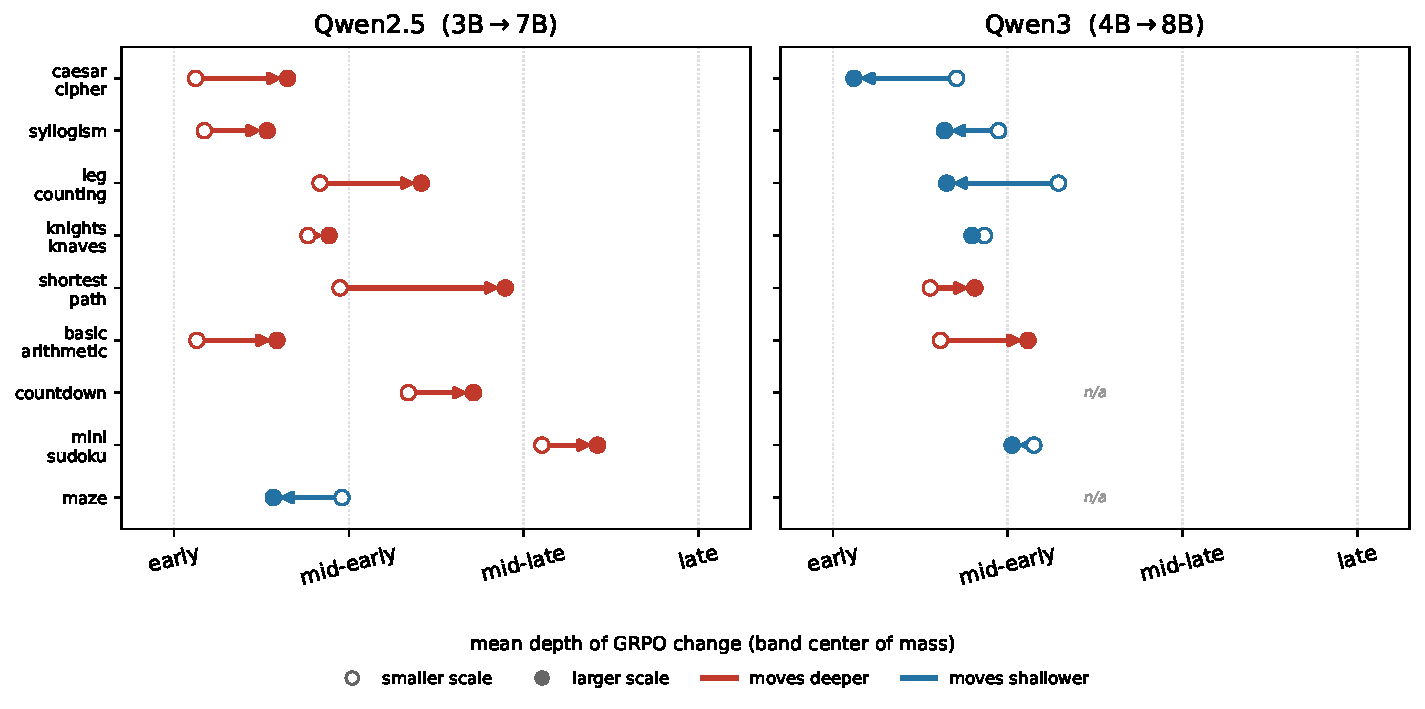
\includegraphics[width=0.92\textwidth]{fig_p3_pertask_depth.pdf}
\caption{\textbf{Per-task depth migration, all tasks} (the all-task version of
Fig.~\ref{fig:p3b}c). Each arrow runs from a family's smaller scale (open marker) to its larger scale
(filled marker) at the task's depth center of mass; red = the change moves deeper with scale,
blue = shallower. \texttt{countdown}@4B (contaminated) and \texttt{maze}@8B (not analyzed) are marked
\emph{n/a}. Qwen2.5 deepens almost universally (maze excepted); Qwen3 deepens only for
\texttt{basic\_arithmetic} and \texttt{shortest\_path}.}
\label{fig:p3pertaskdepth}
\end{figure}

\begin{table}[h]
\centering\small
\caption{\textbf{Depth center of mass per task and scale} (band index, 0 = early $\dots$ 3 = late;
lower is shallower). These are the $x$-coordinates of Fig.~\ref{fig:p3pertaskdepth}. ``--'' marks an
omitted run (\texttt{countdown}@4B contaminated, \texttt{maze}@8B not analyzed).}
\label{tab:p3-pertask-depth}
\begin{tabular}{lrrrr}
\toprule
Task & 3B & 4B & 7B & 8B\\
\midrule
caesar\_cipher    & 0.12 & 0.71 & 0.65 & 0.12\\
syllogism         & 0.17 & 0.95 & 0.53 & 0.64\\
leg\_counting     & 0.84 & 1.29 & 1.42 & 0.65\\
knights\_knaves   & 0.77 & 0.87 & 0.89 & 0.80\\
shortest\_path    & 0.95 & 0.56 & 1.90 & 0.81\\
basic\_arithmetic & 0.13 & 0.61 & 0.59 & 1.12\\
countdown         & 1.34 & --   & 1.71 & 1.24\\
mini\_sudoku      & 2.10 & 1.15 & 2.42 & 1.02\\
maze              & 0.96 & 0.21 & 0.57 & --\\
\bottomrule
\end{tabular}
\end{table}

\end{document}
